\documentclass[usenames,dvipsnames,notes,11pt,aspectratio=169,hyperref={colorlinks=true, linkcolor=blue}]{beamer}
\usepackage{ifthen}
\usepackage{xcolor}
\usepackage{pgfplots}
\usepackage{amsmath}
\usepackage{centernot}
\usepackage{pifont}
\usepackage{tabularx}
\usepackage{makecell}
\usepackage{cuted}
\usepackage{booktabs}
\usepackage{array}
\usepackage{textcomp}
\usepackage{setspace}
\usepackage{xspace}
\usepackage{subcaption}
\usepackage{tikz}
\usepackage{pdfcomment}
%\newcommand{\pdfnote}[1]{\marginnote{\pdfcomment[icon=note]{#1}}}
\newcommand{\pdfnote}[1]{}

\usepackage{pgfpages}
%\setbeameroption{show notes on second screen}


\input ../beamer-style
\input ../std-macros
\input ../macros

\newcommand{\pt}{\partial}

\AtBeginSection[]
{
    \begin{frame}
        \frametitle{Table of Contents}
        \tableofcontents[currentsection]
    \end{frame}
}
\parskip=10pt

\title[CSCI-GA.2590]{Evaluation and Benchmarking}
\author[He He]{He He
}
\institute[NYU]{
    
\includegraphics[height=1cm]{../figures/nyu-logo}\\
}
\date{April 2, 2025}

\begin{document}
\begin{frame}
\titlepage
\end{frame}

\section{Introduction}

\begin{frame}
    {Influence of benchmarks in AI}

    \begin{columns}
        \begin{column}{0.4\textwidth}
            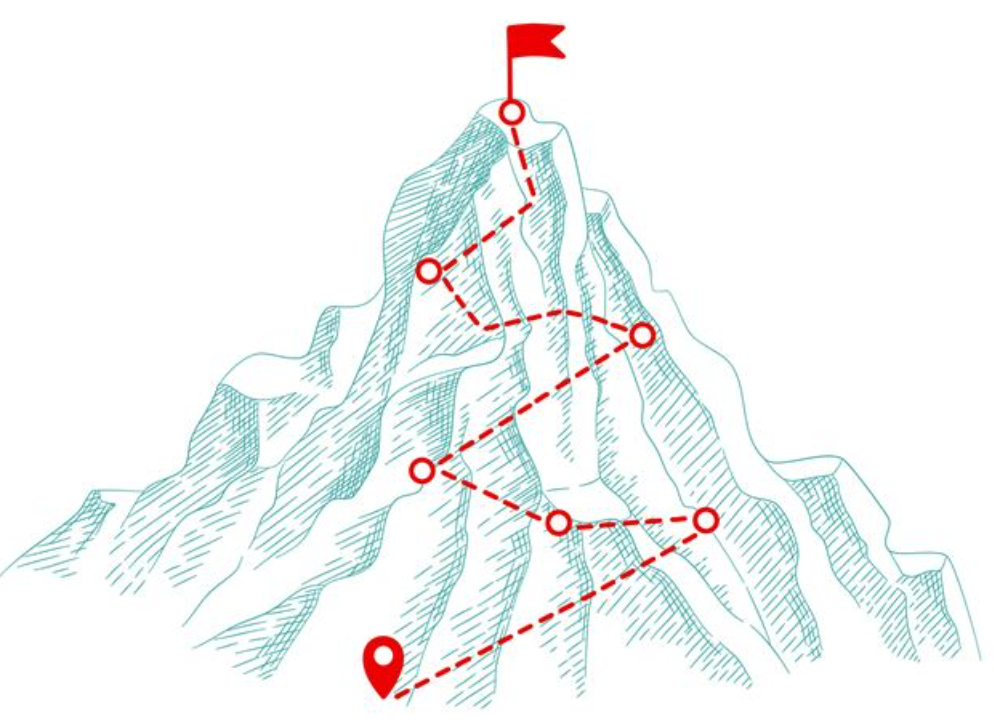
\includegraphics[width=\textwidth]{figures/hill-climbing}
        \end{column}
        \begin{column}{0.6\textwidth}
            \begin{wideitemize}
                \item We cannot make progress if it cannot be measured.
                \item Benchmarks often set the direction of a field.

                \item Key questions answered by a benchmark:
                    \begin{itemize}
                        \item What tasks are \blue{important} and \blue{within reach} now?
                        \item Where do we stand now?
                    \end{itemize}
            \end{wideitemize}
        \end{column}
    \end{columns}
\end{frame}

\begin{frame}
    {Example: ImageNet [Deng et al., 2009]}
    \begin{columns}
        \begin{column}{0.5\textwidth}
            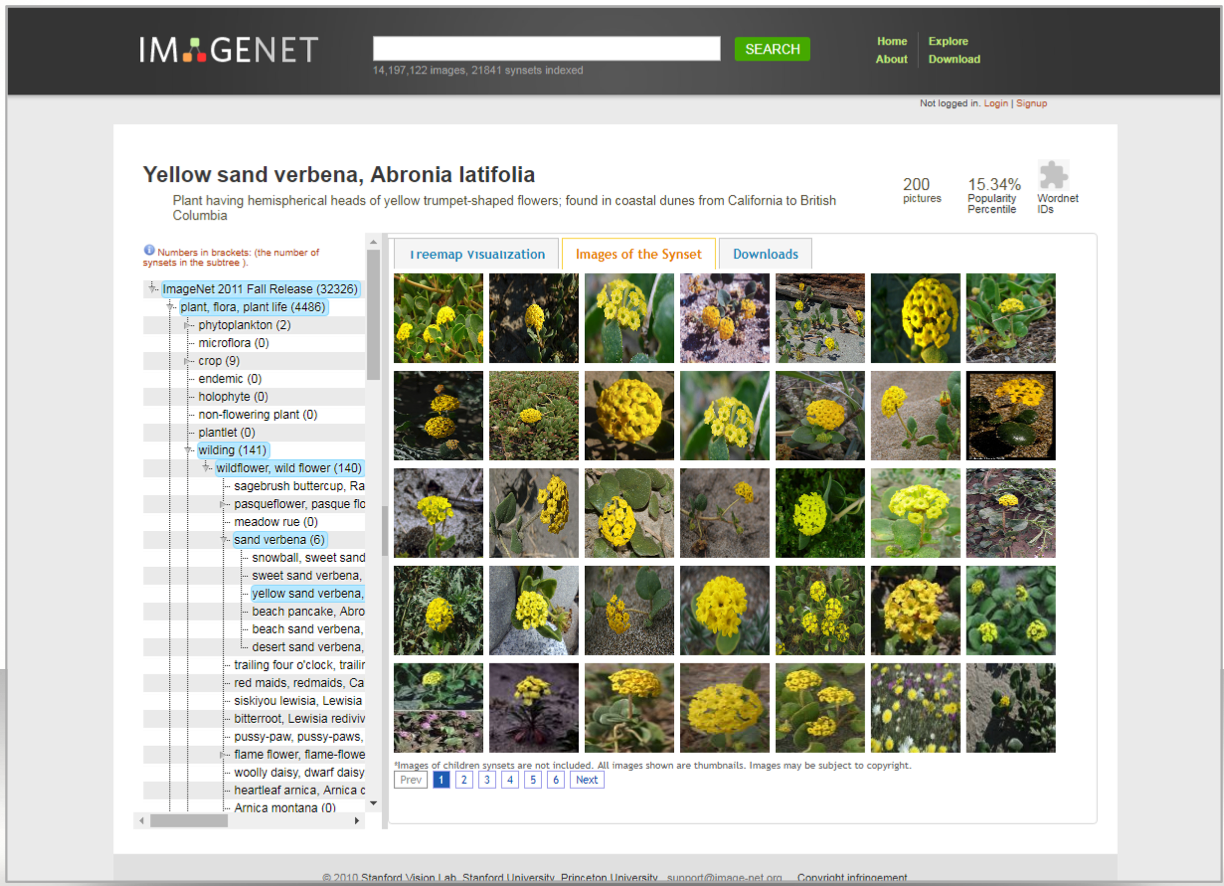
\includegraphics[width=\textwidth]{figures/imagenet}
        \end{column}
        \begin{column}{0.5\textwidth}
            \begin{itemize}
                \item Over 14M labeled images
                \item Data collection leveraged \blue{image search} and \blue{crowdsourcing} (Amazon Mechanical Turk ) \\
                    {\it scale over precision}
                \item Led to the community-wide ILSVRC challenge
                \item The message:\\
                    \textit{Let's learn from lots of data!}
            \end{itemize}
        \end{column}
    \end{columns}
\end{frame}

\begin{frame}
    {Breakthrough of deep learning established by ImageNet}
    \begin{figure}
    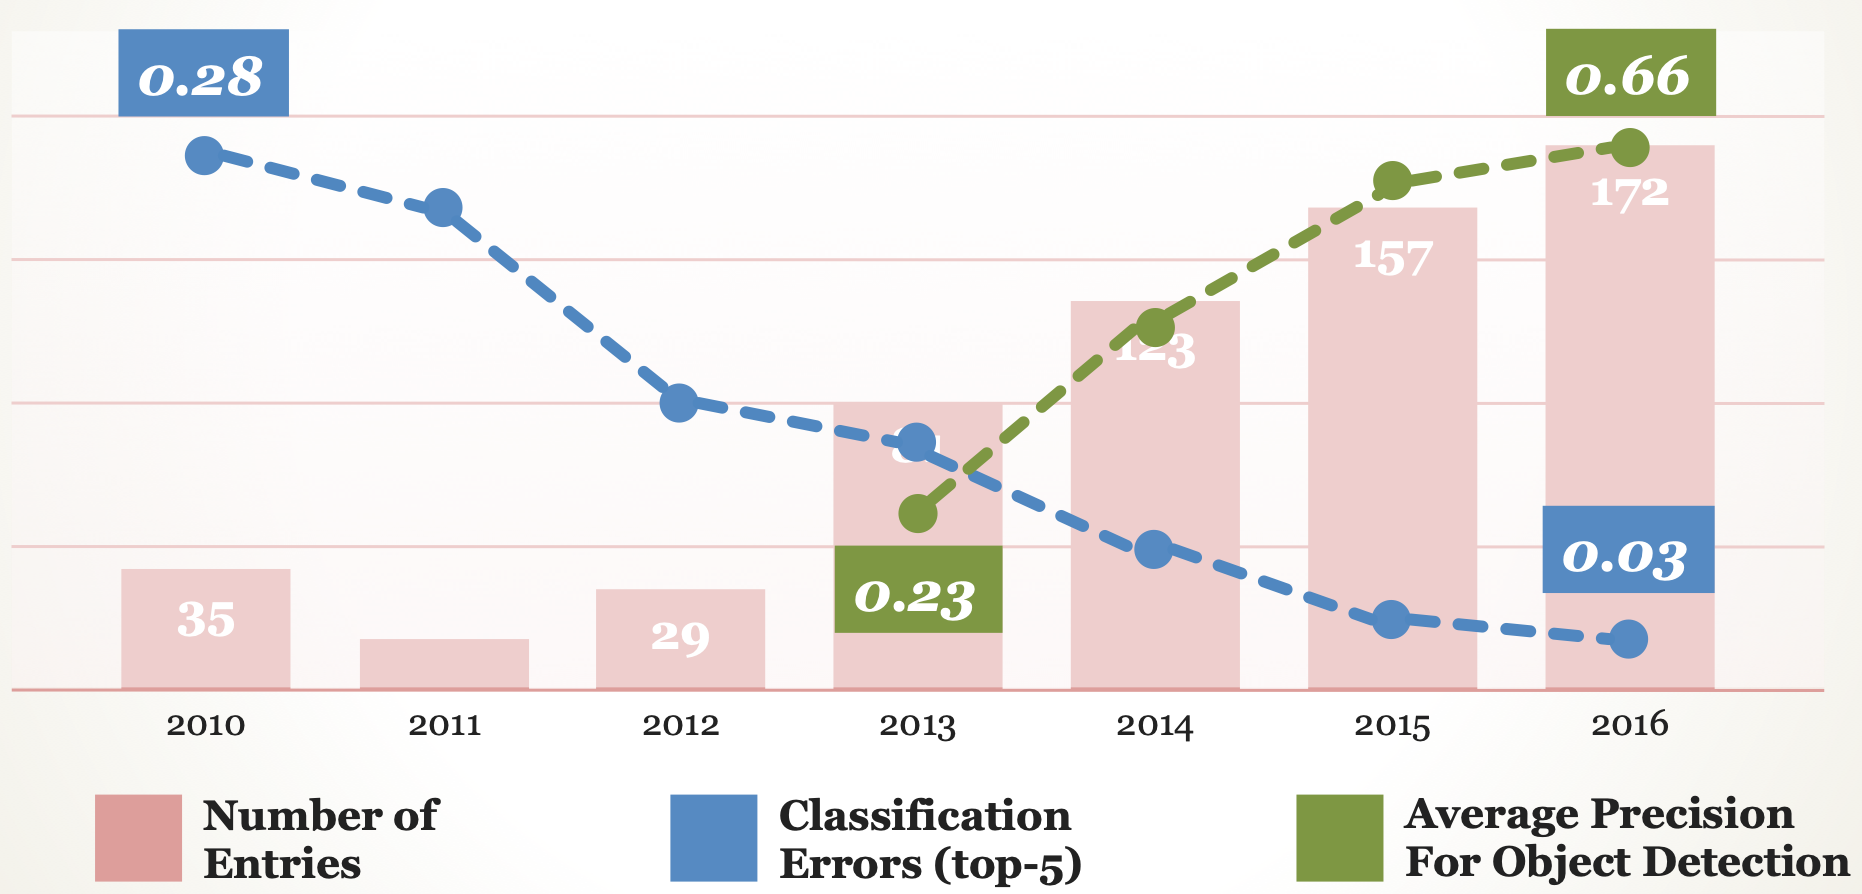
\includegraphics[height=0.6\textheight]{figures/imagenet-progress}
        \caption{From Fei-Fei Li's \href{https://www.image-net.org/static_files/files/imagenet_ilsvrc2017_v1.0.pdf}{slides}}
    \end{figure}
    \vspace{-1em}
    \begin{itemize}
        \item AlexNet \mycite{Krizhevsky et al., 2012} achieved top-1 error rate in ILSVRC 2010.
        \item The result sparked renewed interests in neural netowrks.
    \end{itemize}
\end{frame}

\begin{frame}
    {Example: GLUE [Wang et al., 2019]}
    \begin{figure}
    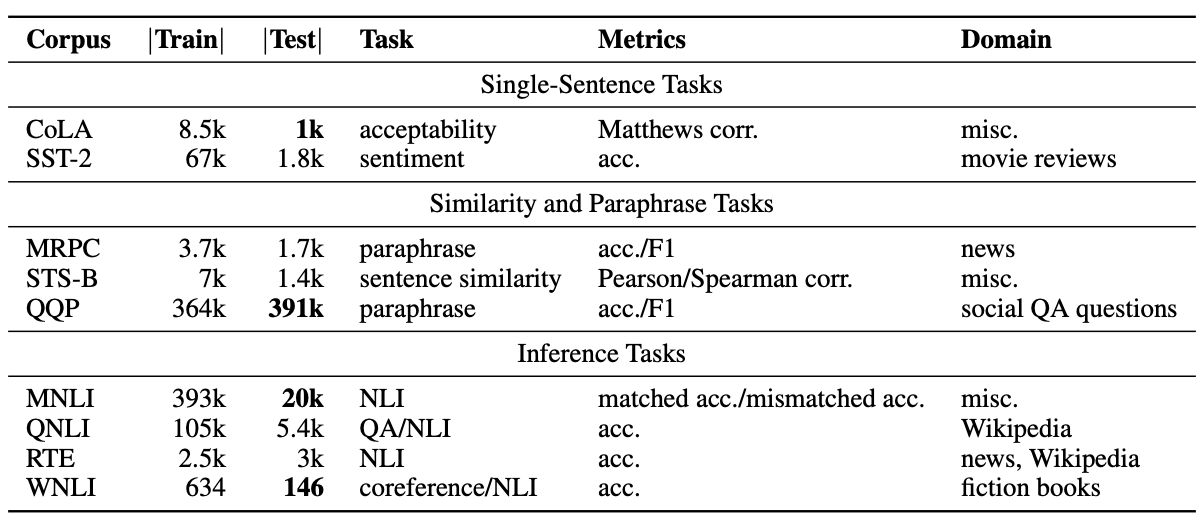
\includegraphics[height=0.6\textheight]{figures/glue}
    \end{figure}
    \vspace{-1em}
    \begin{itemize}
        \item A collection of selected NLU datasets 
        \item Established the breakthrough of pretraining: BERT achieved 7.7 points of improvement
        \item The message: \textit{Let's build general NLU models that adapt to many tasks}
    \end{itemize}
\end{frame}

\section{Evaluating task-specific performance}

\begin{frame}
    {Task-specific evaluation}
    Review of basic classification metrics:
    \begin{wideitemize}
        \item Accuracy: fraction of correct predictions
        \item F1: balances precision and recall---when is this useful?
        \item AUROC: considers trade-off between true positive and false positive across different thresholds
    \end{wideitemize}
\end{frame}

\begin{frame}
    {Evaluating text geneneration tasks}
    \textbf{Task}: given the reference(s) of each source sentence, evaluate the quality of the generated sequences.
    \begin{description}
        \item[Reference 1] It is a guide to action that ensures that the military will forever heed Party commands.
        \item[Reference 2] It is the guiding principle which guarantees the military forces always being under the command of the Party. 
        \item[Candidate 1] It is a guide to action which ensures that the military always obeys the commands of the party.
        \item[Candidate 2] It is to insure the troops forever hearing the activity guidebook that party direct.
    \end{description}

    \pause
    \textbf{Main idea}: good generations should have high overlap with the reference.
\end{frame}

\begin{frame}
    {BLEU: n-gram precision}
    \textbf{First try}: n-gram precision ($x$: input, $c$: candidate, $r$: references)
    $$
    p_n = \frac{
        \sum_{(x,c,r)} \sum_{s\in\text{n-gram}(c)} \BI\pb{s \text{ in } r}
    }
    {
\sum_{(x,c,r)} \sum_{s\in\text{n-gram}(c)} \BI\pb{s \text{ in } c}
    } = \frac{
        \text{\# n-grams in both cand and ref}
    }{
        \text{\# n-grams in cand}
    }
    $$
    \pause
    \textbf{Problem}: can match only a few words in the reference(s)\\
    \begin{description}
        \item[Candidate] the the the the the the the
        \item[Reference 1] The cat is on the mat
        \item[Reference 2] There is a cat on the mat
    \end{description}
    unigram precision = ?

    \pause
    \textbf{Solution}: clip counts to maximum count in the reference(s)
\end{frame}

\begin{frame}
    {BLEU: combine n-gram precision}

    Compute n-gram precision for each $n$ (typically up to 4)

    Then, we need to combine the n-gram precisions.

    Average? Problem: precision decreases roughly exponentially with $n$.

    \pause
    \textbf{Solution}: geometric mean (when $w_n=1/n$)
    $$
    \exp\p{\sum_{i=1}^n w_n \log p_n}
    $$
\end{frame}

\begin{frame}
    {BLEU: brevity penalty}

    Problem with precision: ``One who does nothing also does nothing wrong''

    \begin{description}
        \item[Candidate] of the 
        \item[Reference 1] It is the guiding principle which guarantees the military forces always being under the command of the Party. 
        \item[Reference 2] It is the practical guide for the army always to heed the directions of the party.
    \end{description}

    Why not use recall? %with \textit{multiple} references?
    \pdfnote{
       BLEU does not use recall because the notion of recall is unclear when simultaneously matching against multiple reference translations (rather than a single reference).  
    }
\end{frame}

\begin{frame}
    {BLEU: brevity penalty}

    %A good translation must match the reference in:\\
    %\begin{description}
    %    \item[word choice] captured by precision
    %    \item[word order] capture by n-gram
    %    \item[length] ?
    %\end{description}

    \textbf{candidate length} $C=\sum_{(x,c,r)} \text{len}(c)$

    \textbf{reference length} $R=\sum_{(x,c,r)} \argmin_{a\in\pc{\text{len}(r_1),\ldots,\text{len}(r_k)}} |a-\text{len}(c)|$\\
    \begin{itemize}
        \item Use the reference whose length is closest to the candidate
    \end{itemize}

    \textbf{Brevity penalty} $BP =
    \begin{cases}
        1 & \text{if } c \ge r \quad \text{no penalty}\\
        e^{1-R/C} & \text{if } c < r \quad \text{downweight score}
    \end{cases}
    $
\end{frame}

\begin{frame}
    {BLEU}
    Putting everything together:
    \begin{align*}
        \text{BLEU} &= BP\cdot \exp\p{\sum_{n=1}^N w_n \log p_n} \\
        %\log \text{BLEU} &= \min(1-\frac{R}{C}, 0) + \sum_{n=1}^N w_n \log p_n
    \end{align*}
    \vspace{-2em}

    \pause
    A good translation should match the references in word choice, word order, and length. (How is each part captured by BLEU?)

    \pause
    Practicalitis:\\
    \begin{itemize}
        \item Both precision and the brevity penalty are computed at the \emph{corpus level}.
        \item Need smoothing for sentence-level BLEU.
        \item Good correlation with human evaluation for MT (typically $n=4$).
    \end{itemize}
\end{frame}

\begin{frame}
    {ROUGE}
    \textbf{Task}: given a candidate summary and a set of reference summaries, evaluate the quality of the candidate.

    \textbf{ROUGE-n}: n-gram recall\\
    \begin{itemize}
        \item Encourage content coverage 
    \end{itemize}

    \textbf{ROUGE-L}: measures longest common subsequence between a candidate and a reference (doesn't require consecutive match.)\\
    \begin{itemize}
        \item Precision $ = LCS(c, r) / \text{len}(c)$
        \item Recall $ = LCS(c, r) / \text{len}(r)$
        \item F-measure $ = \frac{(1+\beta^2)RR}{R + \beta^2 P}$
    \end{itemize}
\end{frame}

\begin{frame}
    {Automatic evaluation metrics for generation}
    n-gram matching metrics (e.g. BLEU, ROUGE)\\
    \begin{itemize}
        \item Measures exact match with reference; interpretable.
        \item Do not consider semantics.
        \item Mainly used for machine translation
    \end{itemize}

    \pause
    Embedding-based metrics (e.g. BERTScore, MAUVE)\\
    \begin{itemize}
        \item Measures similarity to the reference in an embedding space.
        \item Captures synonyms and simple paraphrases
        \item Results are often correlated with n-gram matching metrics
    \end{itemize}

    \pause
    \textbf{Human evaluation} is still needed for\\
    \begin{itemize}
        \item Is the generation correct? e.g. faithfulness (summarization), adequacy (MT).
        \item Is the story/dialogue interesting, informative, engaging?
    \end{itemize}
\end{frame}

\begin{frame}
    {Evaluating coding ability}
        
    {\bf HumanEval}: generating code given docstrings; human-written solution and unit tests
    \begin{figure}
        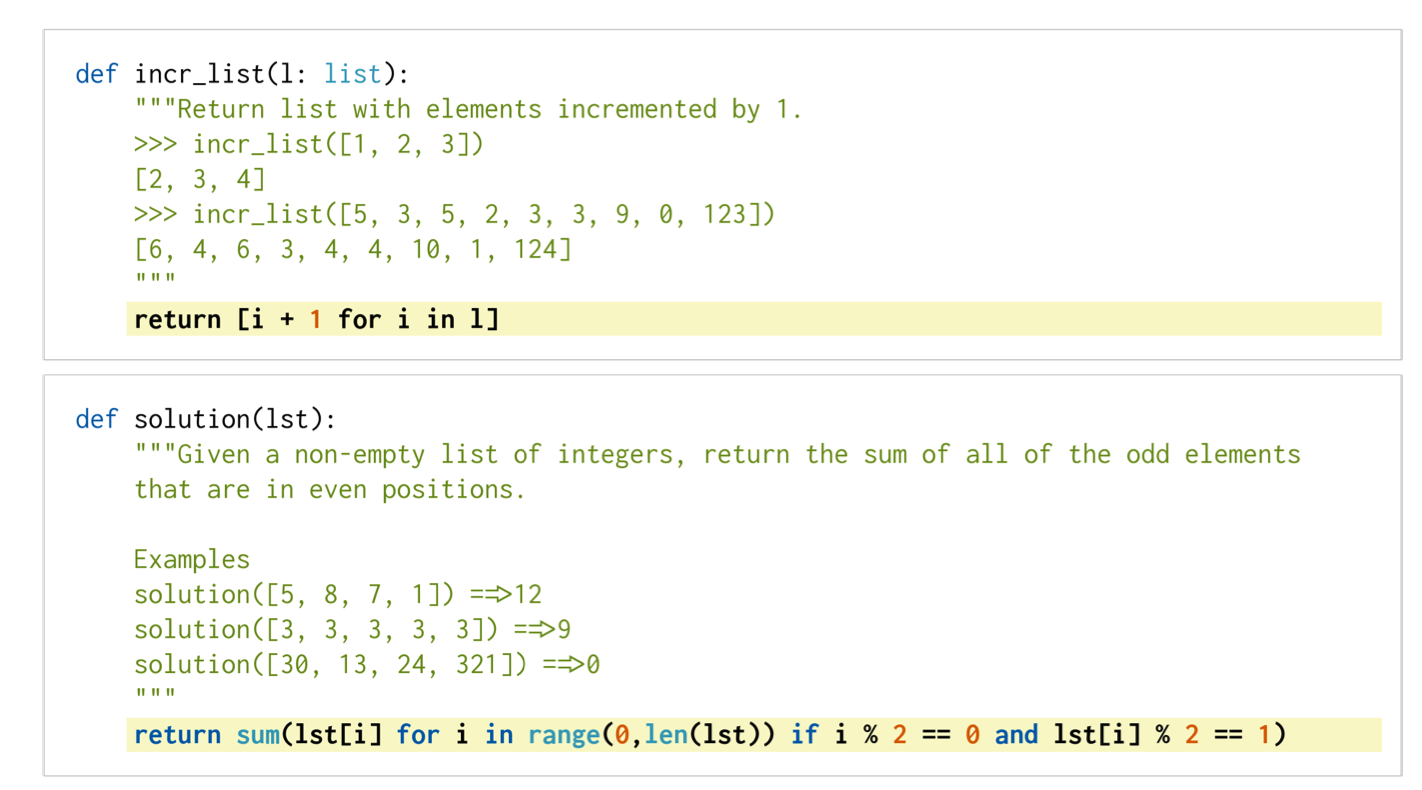
\includegraphics[width=0.7\textwidth]{figures/humaneval}
        \caption{[Chen et al., 2021]}
    \end{figure}
\end{frame}

\begin{frame}
    {Metrics}
    {\bf pass@k}: consider the output correct if at least one of the $k$ samples is correct\\
    \begin{itemize}
        \item Use larger temperatur for large $k$
    \end{itemize}
    \begin{figure}
        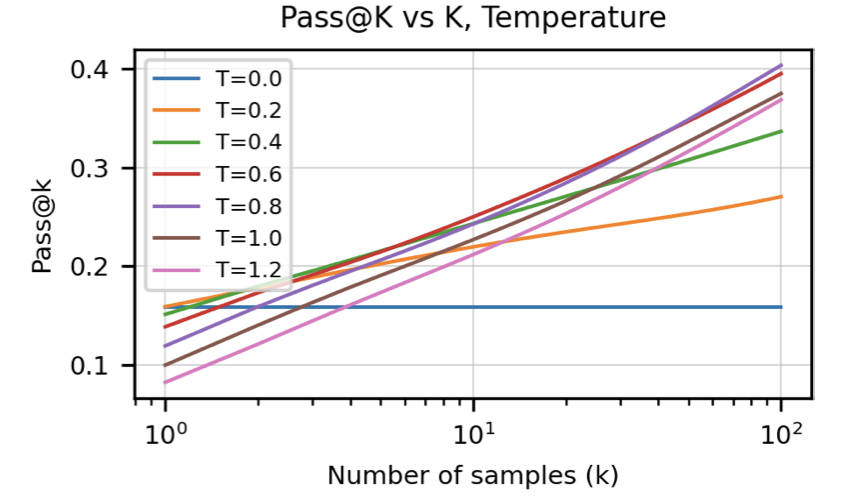
\includegraphics[width=0.5\textwidth]{figures/pass-k}
    \end{figure}
\end{frame}

\section{Evaluating general capabilities}

\begin{frame}
    {Challenges in evaluating LLMs}
    What are challenges in evaluating LLMs like ChatGPT? \pause
    \begin{wideitemize}
        \item Many use cases (coding, writing, knowledge retrieval etc.) 
        \item Open-ended, long-form generation
        \item Data contamination: how do we know if our test data is unseen? 
    \end{wideitemize}
\end{frame}

\begin{frame}
    {Expanding the set of tasks}
    \begin{wideitemize}
        \item Problem: models are no longer trained for a single task
        \item Solution: test on a collection of tasks---a benchmark
        \item Challenge: find challenging {\it and} easy-to-evaluate data sources
            \begin{itemize}
                \item Data source: exisiting datasets, exams, expert-written questions
                \item Evaluation: multiple choice or numerical answers 
            \end{itemize}
    \end{wideitemize}
\end{frame}

\begin{frame}
    {Massive multitask language understanding}
    MMLU \mycite[]{[Hendrycks et al., 2021]}: MC questions covering 57 academic topics evaluated by accuracy\\
    \begin{itemize}
        \item Current frontier LMs approach human-level (~85\% to 90\%)
        \item Mainly measures knowledge retrieval and simple reasoning 
    \end{itemize}
    \begin{figure}
        
\includegraphics[width=0.7\textwidth]{figures/mmlu}
    \end{figure}
\end{frame}

\begin{frame}
    {Other similar benchmarks}
    \begin{wideitemize}
        \item {\bf BIG-bench}: the most broad benchmark
            \begin{itemize}
                \item Methodology: crowdsource tasks from the community 
                \item Limitation: Tasks vary in quality and difficulty; some tasks may be niche, e.g., inferring movie title from emojis
            \end{itemize}
        \item {\bf HELM}: multi-dimensional and transparent evaluation of LMs
            \begin{itemize}
                \item Evaluate robustness, calibration, fairness, etc. in addition to correctness---harder to distill into a sipmle leaderboard
                \item Compare all models on the same set of data and release model outputs
            \end{itemize}
    \end{wideitemize}
\end{frame}

\begin{frame}
    {Do we really need to test on this many tasks?}
    \begin{columns}
        \begin{column}{0.5\textwidth}
            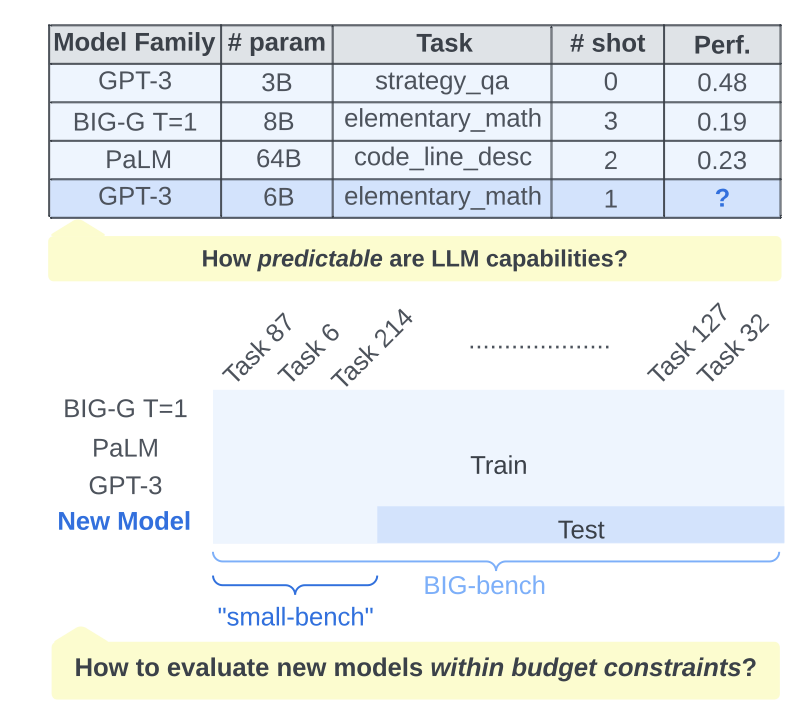
\includegraphics[width=\textwidth]{figures/cap-pred}
        \end{column}
        \begin{column}{0.5\textwidth}
            \begin{wideitemize}
                \item Train on a small set of tasks can predict performance on other tasks
                \item Key is to find a set of diverse and representative tasks
                \item Open question: can we predict ``emergent'' abilities?
            \end{wideitemize}
        \end{column}
    \end{columns}
\end{frame}

\begin{frame}
    {The benchmark saturation problem}
    \begin{figure}
        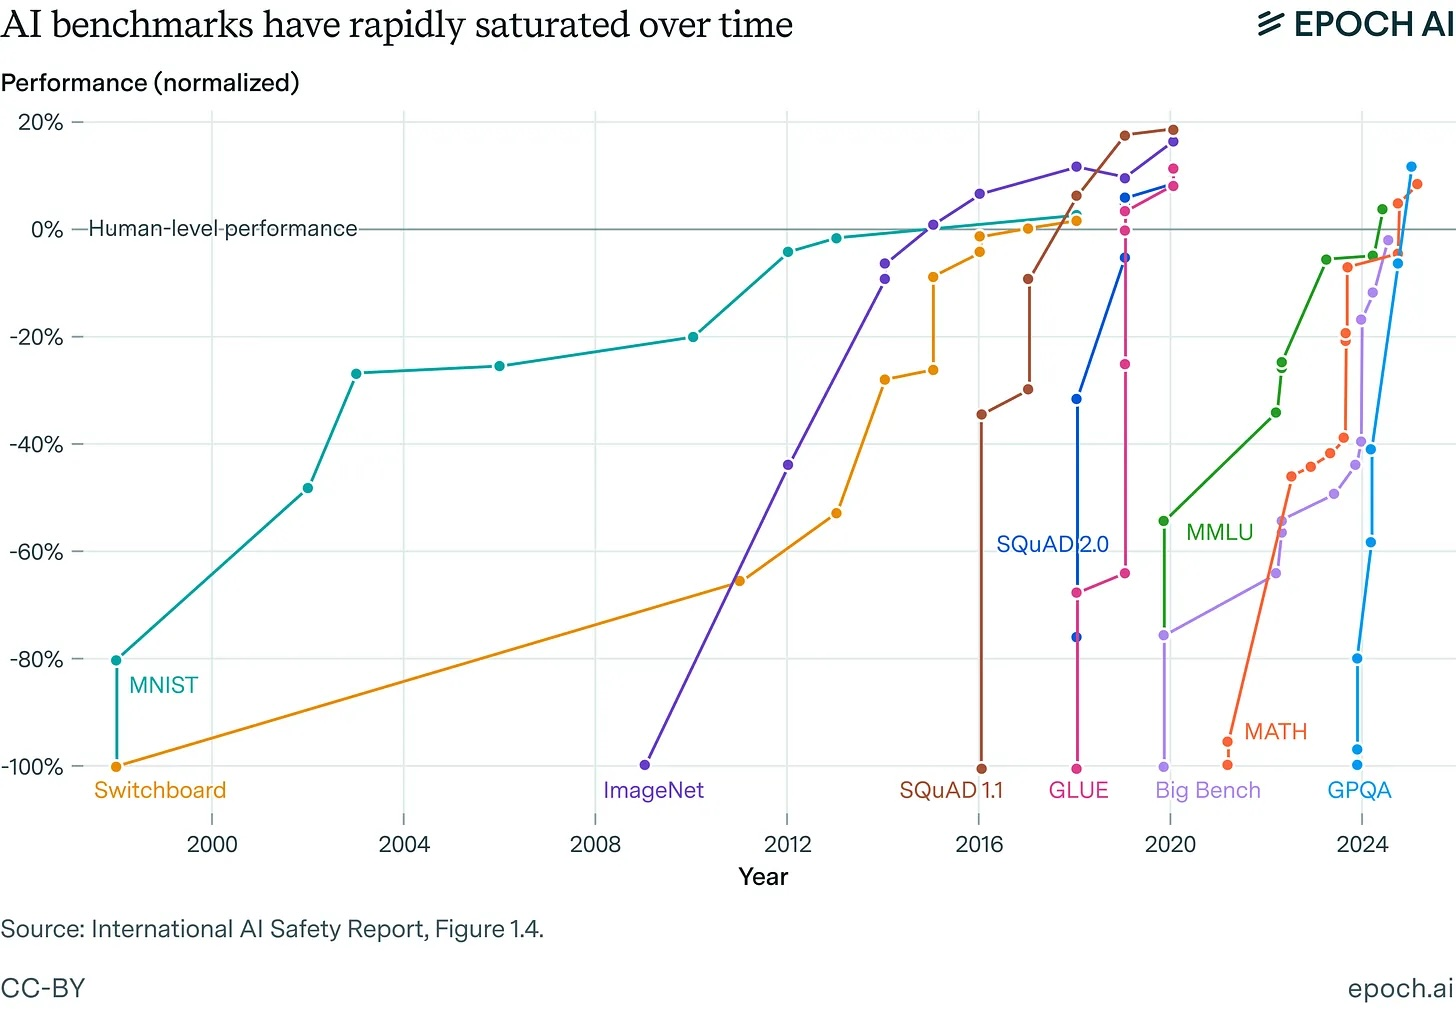
\includegraphics[width=0.8\textwidth]{figures/saturation}
    \end{figure}
\end{frame}

\begin{frame}
    {Moving towards real-world evaluation}
    SWE-Bench \mycite[https://arxiv.org/pdf/2310.06770]{[Jimenez et al., 2024]}
    \begin{figure}
        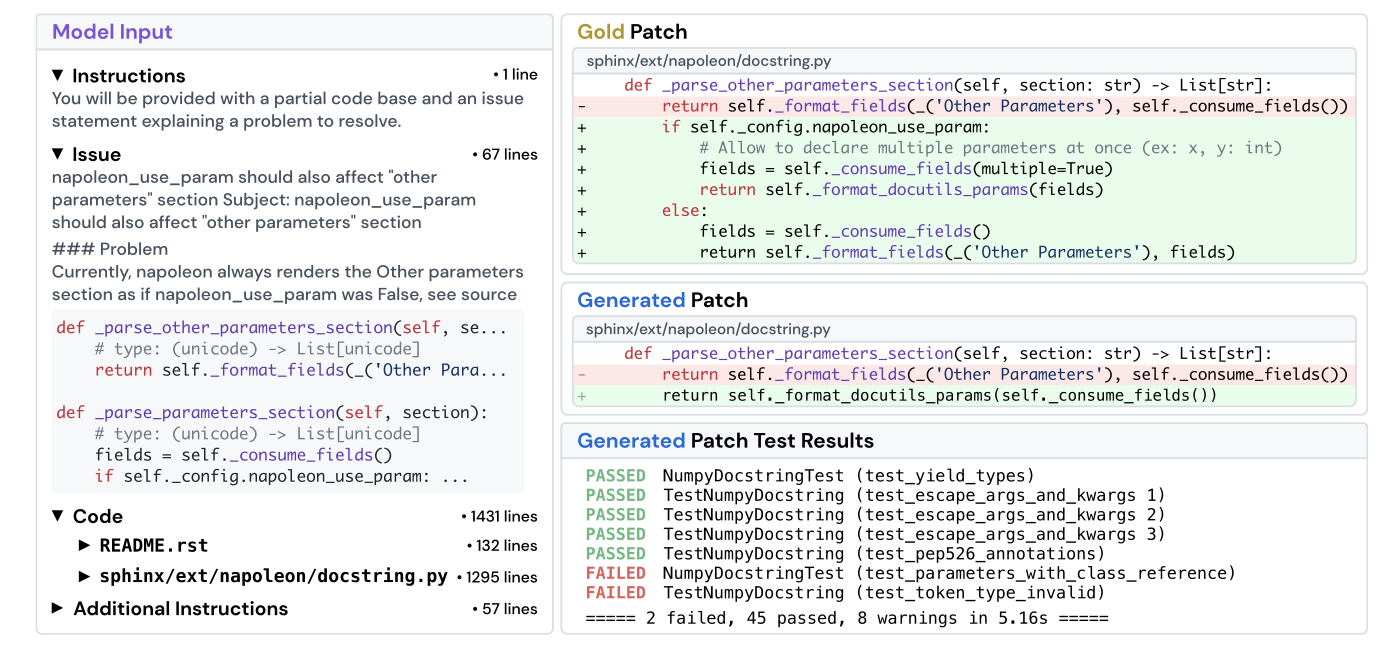
\includegraphics[width=0.8\textwidth]{figures/swe}
    \end{figure}
\end{frame}

\begin{frame}
    {Moving towards real-world evaluation}
    SWE-Lancer \mycite[https://arxiv.org/pdf/2502.12115]{[Miserendino et al., 2025]}
    \begin{figure}
        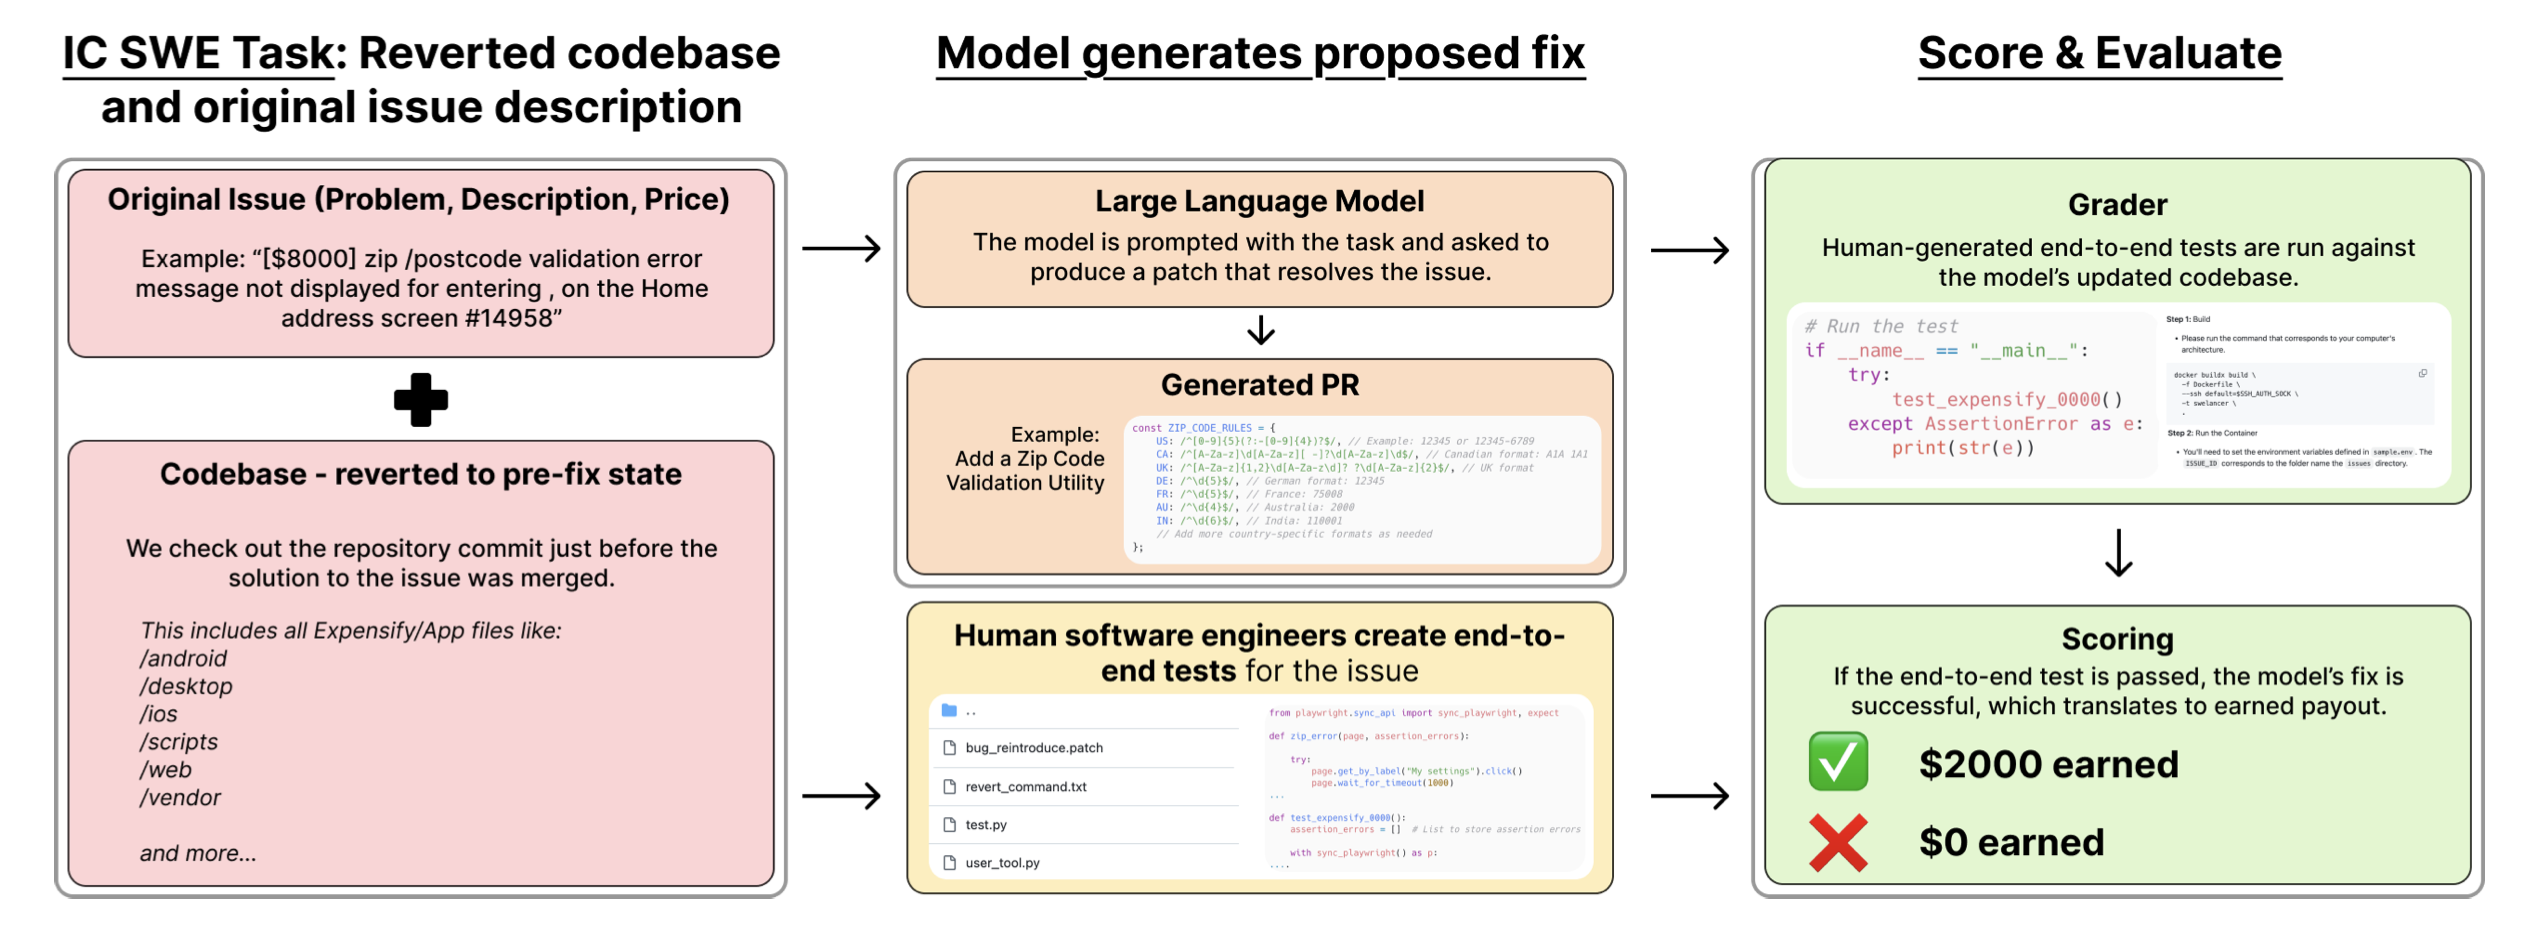
\includegraphics[width=0.9\textwidth]{figures/swe-lancer}
    \end{figure}
\end{frame}

%\begin{frame}
%    {Testing on real unseen data}
%    TODO: Livebench
%\end{frame}

\section{Alternative evaluation strategies}

\begin{frame}
    {Motivation}
    \begin{wideitemize}[<+->]
        \item Benchmarks are suitable for easy-to-evaluate tasks with determinant answers
        \item But we also care about more open-ended tasks and interactive tasks
            \begin{itemize}[<.->]
                \item User preference, helpfulness, etc.
            \end{itemize}
        \item How to evaluate without references?
            \begin{itemize}[<.->]
                \item Use other judges: models, crowdworkers, experts
                \item Use environment feedback: games
            \end{itemize}
    \end{wideitemize}
\end{frame}

\begin{frame}
    {Rank model by user preference}

    {\bf ChatbotArena}: live benchmark based on head-to-head comparison\\
    \begin{itemize}
        \item  {\bf MT Bench}: fixed prompt set + LLM as a judge
    \end{itemize}
    \begin{figure}
        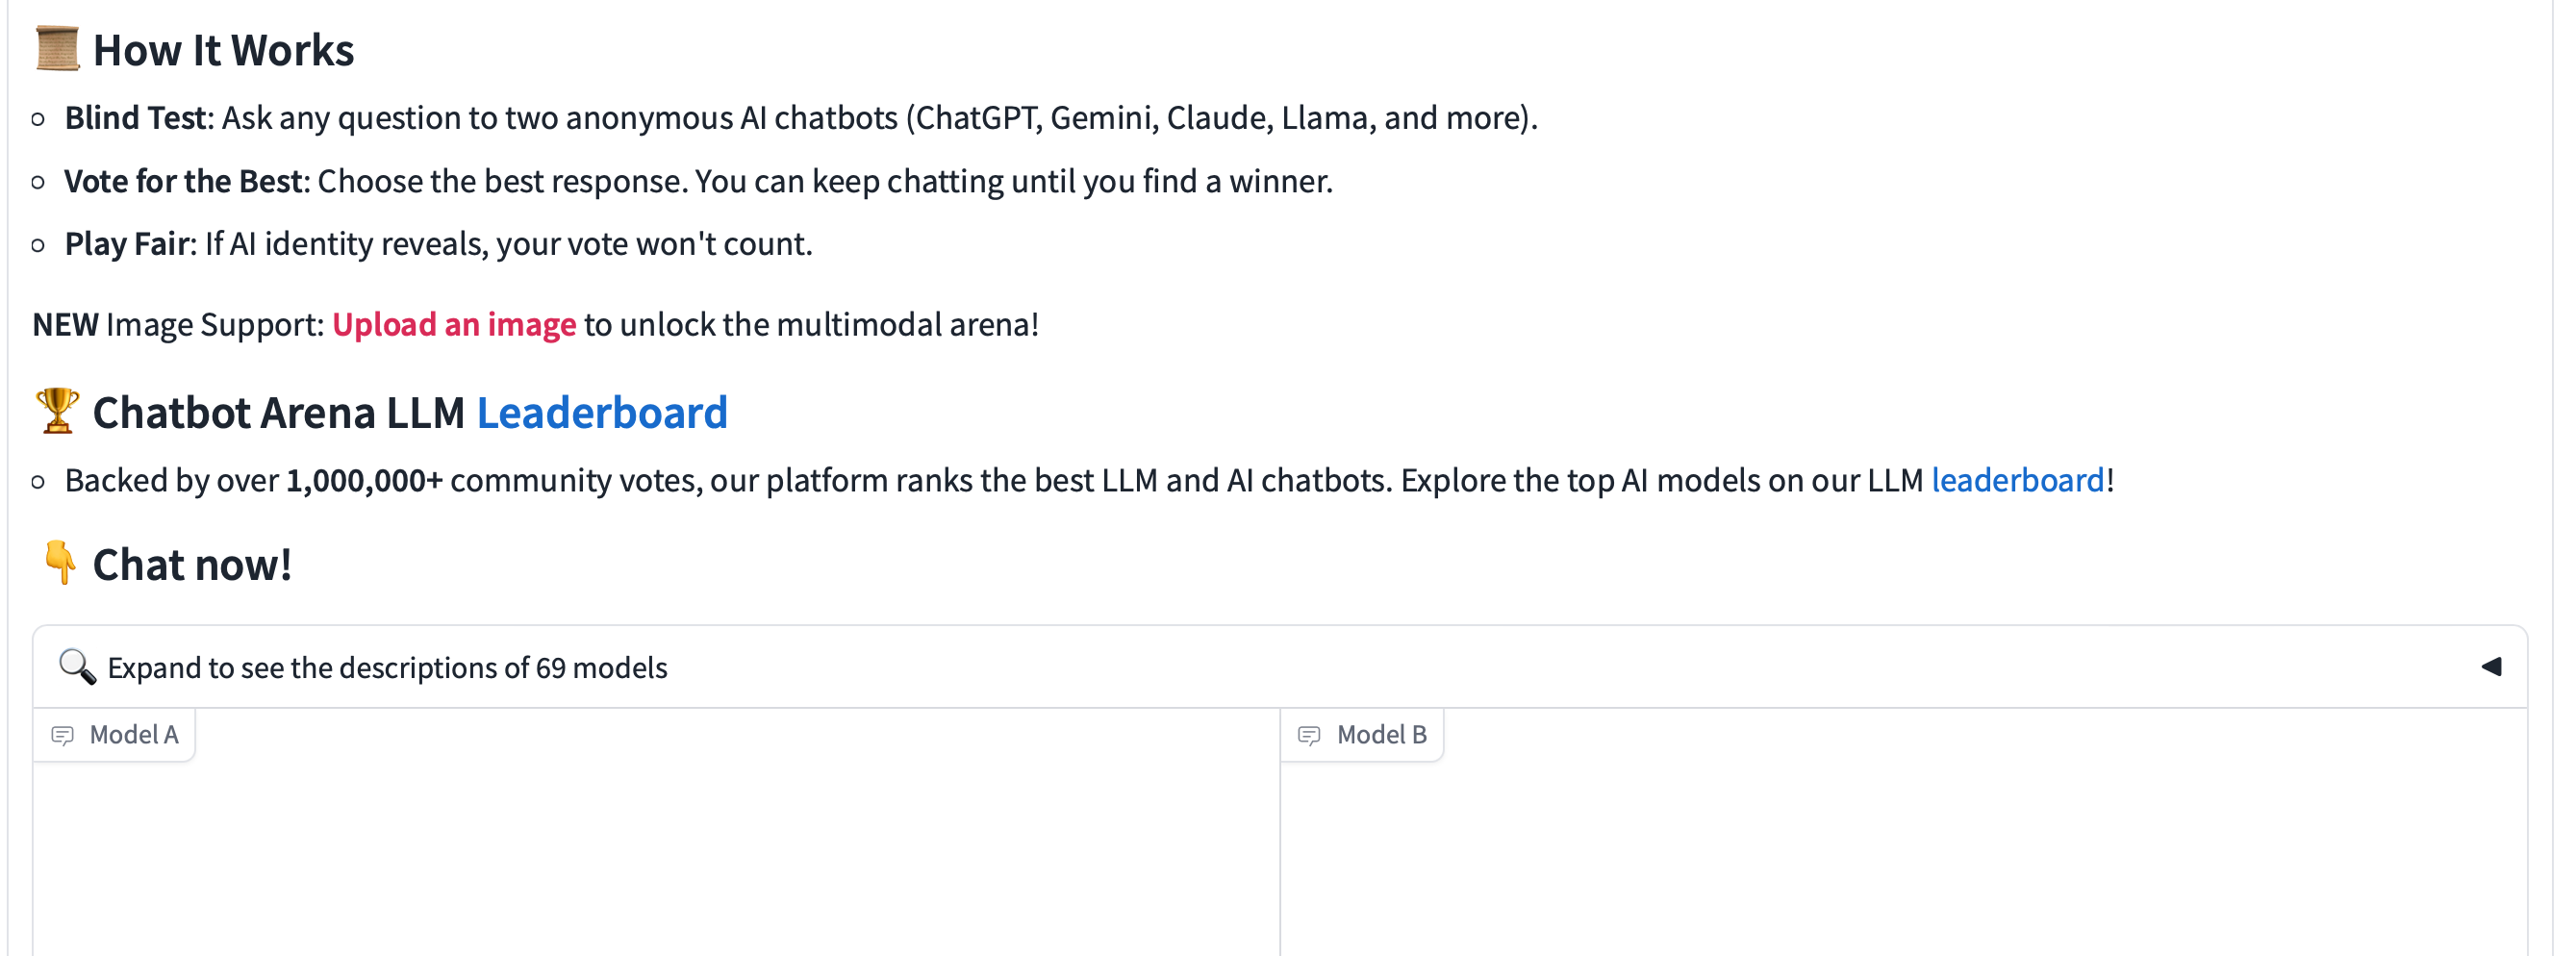
\includegraphics[width=0.9\textwidth]{figures/arena-chat}
        \caption{\url{https://lmarena.ai}}
    \end{figure}
\end{frame}

\begin{frame}
    {Rank model by user preference}

    Challenge: how to produce a ranking based on pairwise comparisons?
    \begin{figure}
        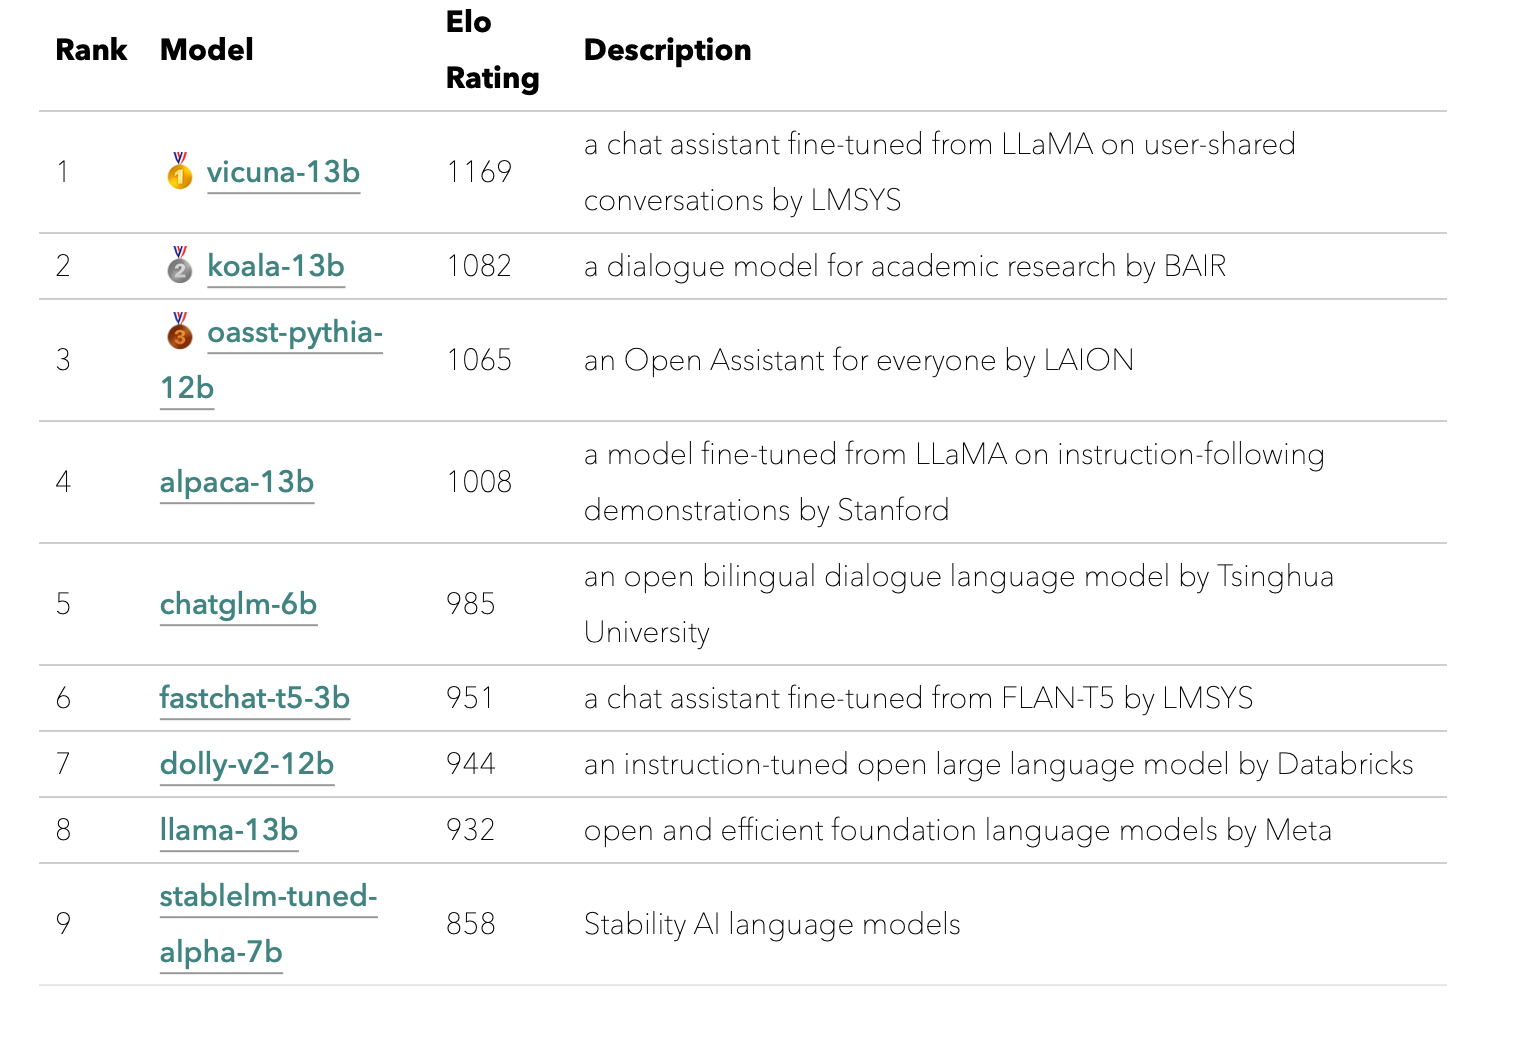
\includegraphics[width=0.7\textwidth]{figures/arena-rank}
    \end{figure}
\end{frame}

\begin{frame}
    {Ranking LLMs}
    \begin{wideitemize}[<+->]
        \item The ideal metric is {\bf average win rate}, but it requires data for every pair of models---expensive!
        \item {\bf Elo rating}: estimate expected win rate given sequential comparisons of model A and model B
            \begin{align}
                E_A &= \frac{1}{1 + 10^{(R_B-R_A)/400}} \\
                S_A &\leftarrow R_A + K\cdot (S_A - E_A)
            \end{align}
            \begin{itemize}[<.->]
                \item $E_A$: expected win rate $p(A \succ B)$
                \item $R_B, R_A$: current ratings of A and B
                \item $S_A$: observed data---actual win (1) or lose (0)
                \item Update: similar to SGD 
            \end{itemize}
    \end{wideitemize}
\end{frame}

\begin{frame}
    {Hack ChatbotArena}
    How would you hack ChatbotArena?\pause
    \begin{figure}
        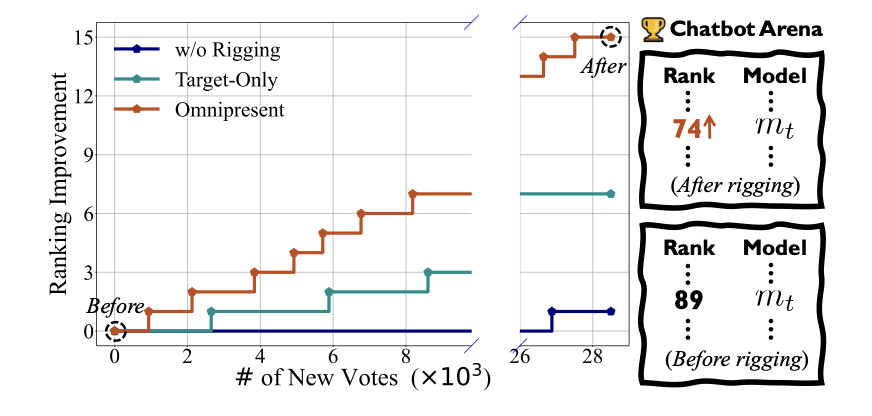
\includegraphics[width=0.6\textwidth]{figures/rigging}
        \caption{\mycite[https://arxiv.org/abs/2501.17858]{[Min et al., 2025]}}
    \end{figure}
    \vspace{-1em}
    \pause
    \begin{itemize}
        \item Detect the target model output
        \item Rate target model output as winning
        \item Detect and rate other models' output to improve target model ranking
    \end{itemize}

\end{frame}

\begin{frame}
    {Limitations of human judges}

    What are limitations of using human feedback?\pause
    \begin{wideitemize}
        \item Expensive %: TODO: example cost on ChatbotArena?
        \item Preference does not equal to correctness
            \begin{itemize}
                \item Humans may prefer human-pleasing but incorrect answers %TODO example
            \end{itemize}
        \item Reproducibility
    \end{wideitemize}
\end{frame}

\begin{frame}
    {LLM as a judge}

    {\bf AlpacaEval}: use LLMs to simulate human preference
    
    \begin{figure}
        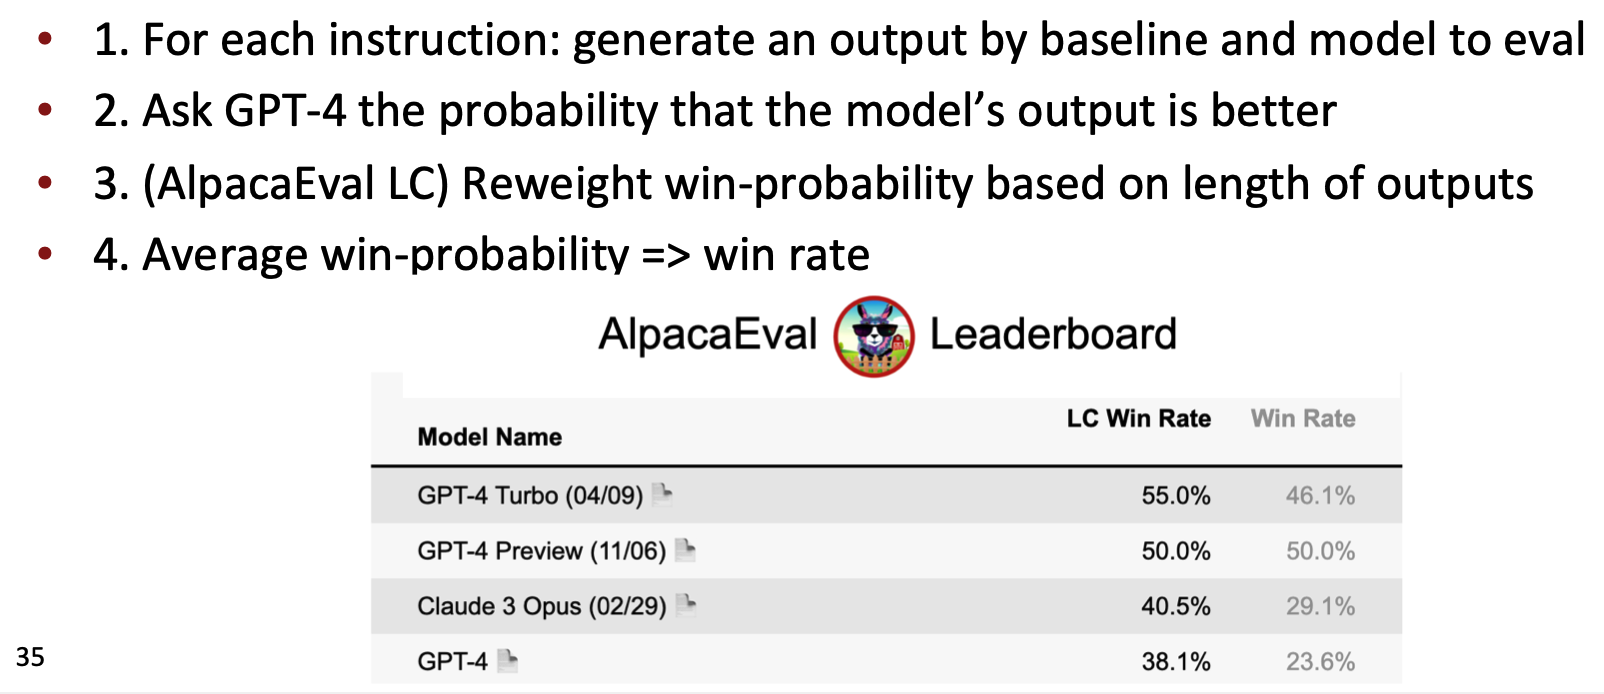
\includegraphics[width=0.8\textwidth]{figures/alpacaeval}
        \caption{From Yann Dubois' slides}
    \end{figure}
\end{frame}

\begin{frame}
    {LLM as a judge}
    High correlation with human 
    \begin{figure}
        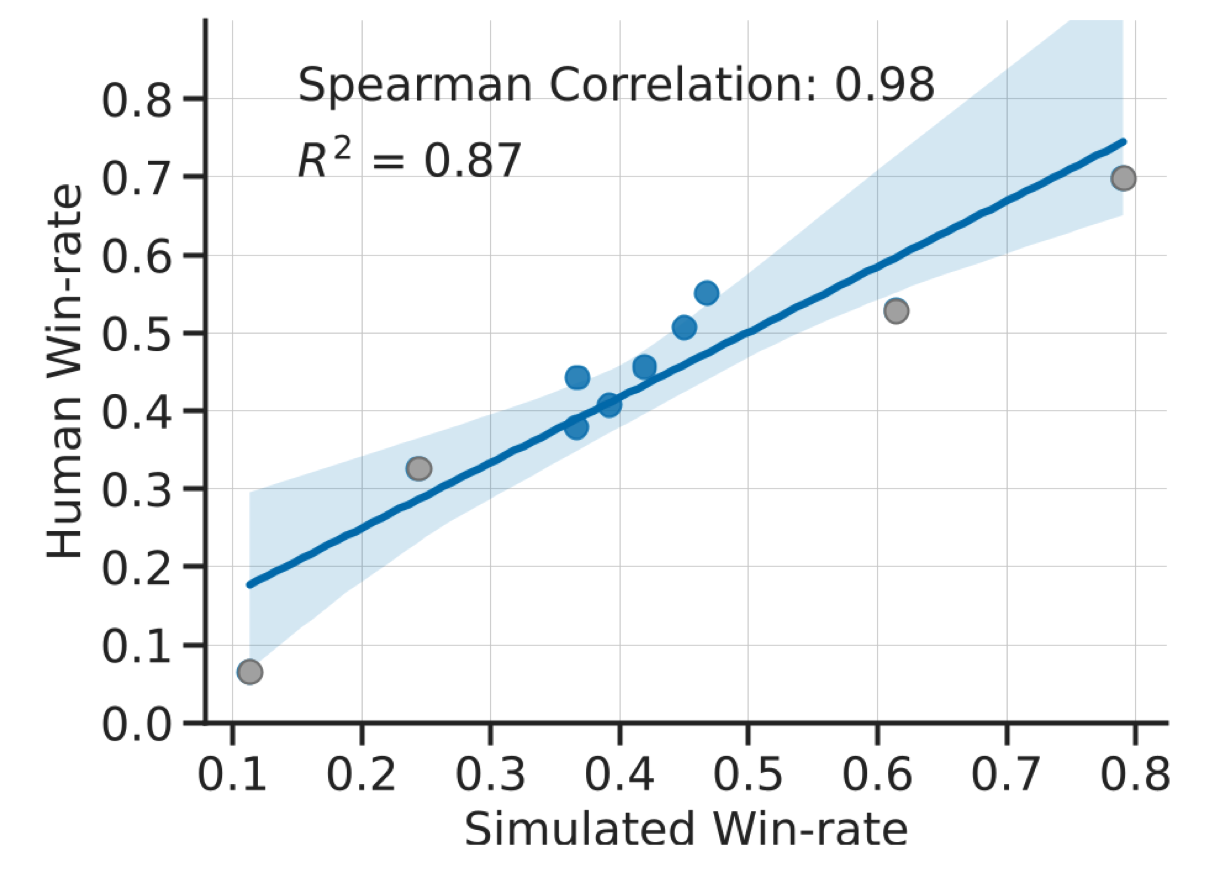
\includegraphics[width=0.6\textwidth]{figures/alpacaeval-corr}
    \end{figure}
\end{frame}

\begin{frame}
    {Limitations of LLM as a judge}
    LLM as a judge is scalable and fast, which allows for rapic iteration. What could go wrong?\pause

    {\bf Position bias}: when comparing two answers, the order of the answers may bias the outcome
    \begin{figure}
        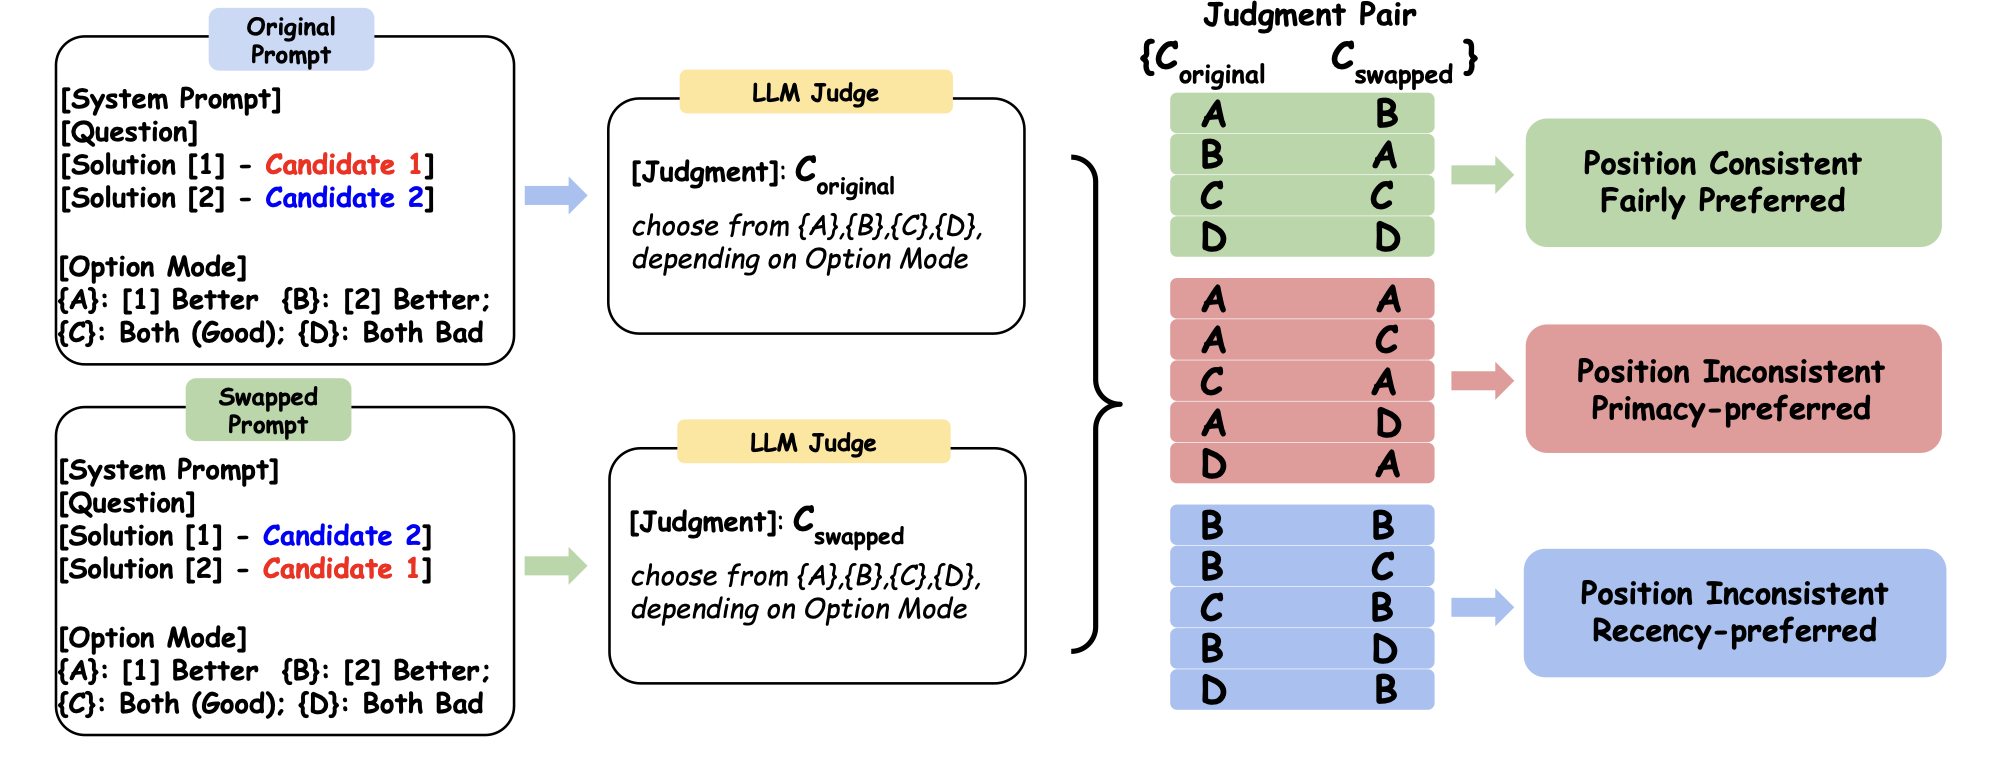
\includegraphics[height=0.5\textheight]{figures/pos-bias}
        \caption{\mycite[https://arxiv.org/pdf/2406.07791]{[Shi et al., 2024]}}
    \end{figure}

    Always randomize answer order when providing two answers
\end{frame}

\begin{frame}
    {Limitations of LLM as a judge}
    
    {\bf Length bias}:
    increasing answer length can improve model rating
    \begin{figure}
        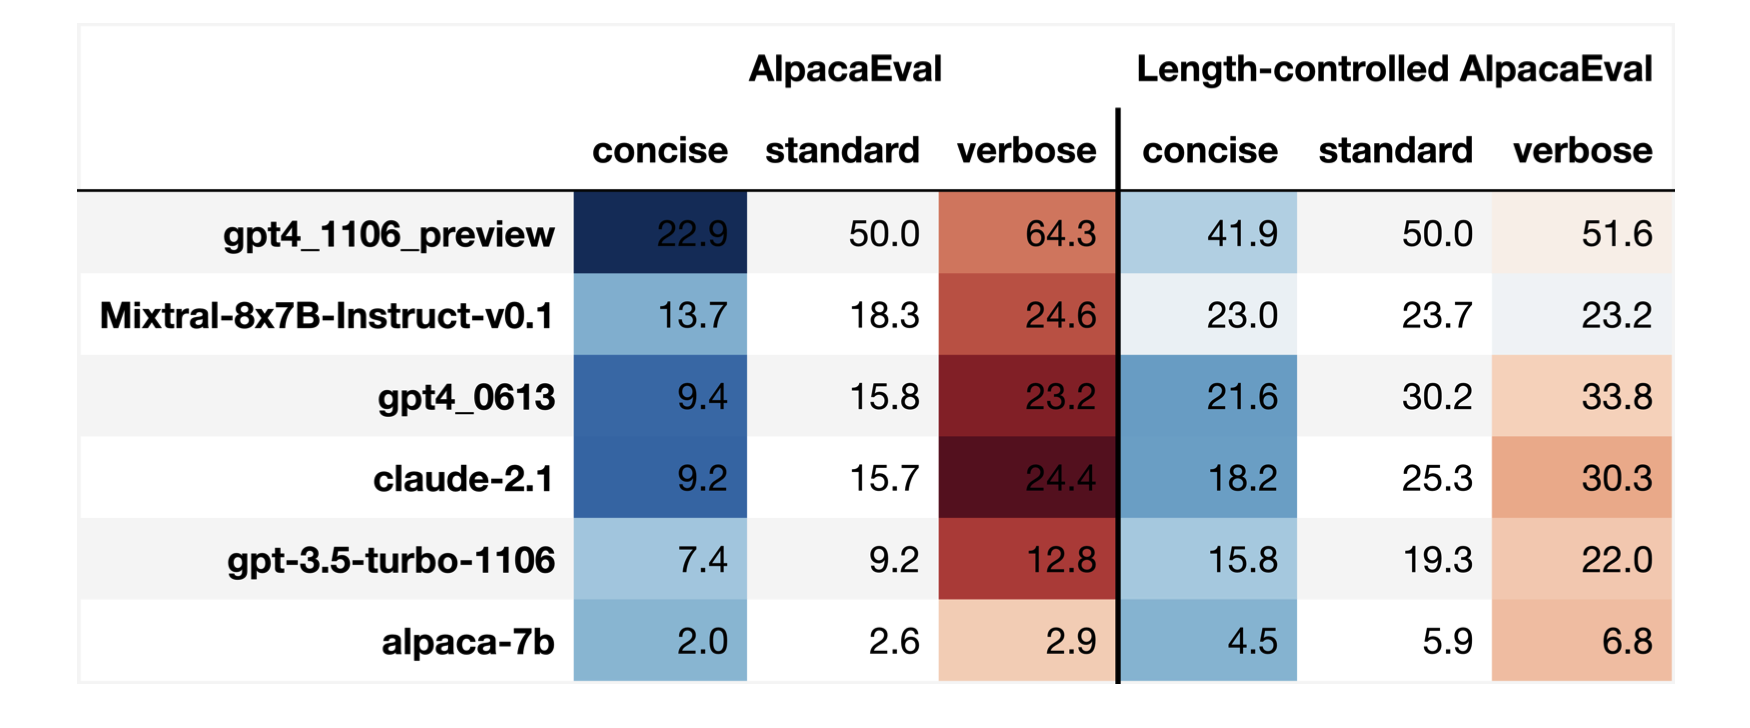
\includegraphics[width=0.7\textwidth]{figures/alpacaeval-length}
    \end{figure}
    Control for length: estimating contribution from different factors (model, length, instruction)
\end{frame}

\begin{frame}
    {Limitations of LLM as a judge}

    {\bf Self-preference bias}: LM favors its own generations \\
    \begin{figure}
        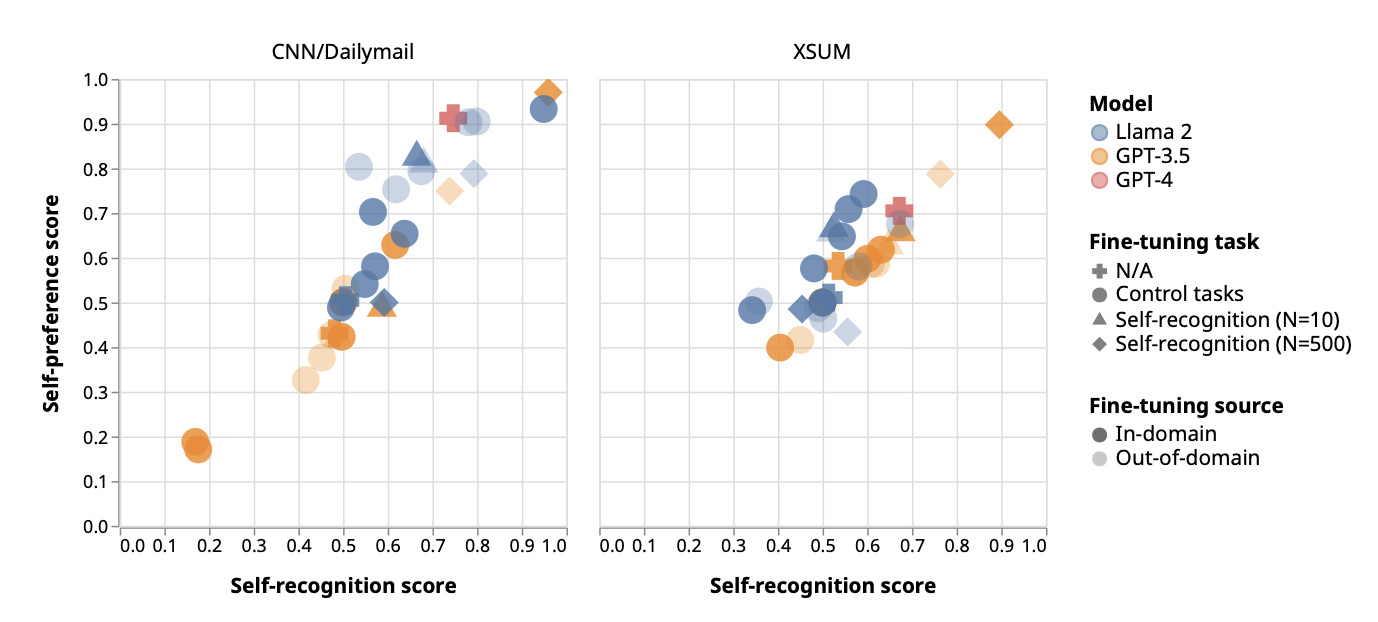
\includegraphics[width=0.8\textwidth]{figures/self-pref}
        \caption{\mycite[https://proceedings.neurips.cc/paper_files/paper/2024/file/7f1f0218e45f5414c79c0679633e47bc-Paper-Conference.pdf]{[Panickssery et al., 2024]}}
    \end{figure}

\end{frame}

\begin{frame}
    {Evaluating models beyond accuracy}

    %Linguists, cognitive scientists: \textbf{interpretability}\\
    %\begin{itemize}
    %    \item How does the model make predictions? Is it human-like?
    %\end{itemize}
    %\pause

    Practitioners: \textbf{efficiency}, \textbf{robustness}\\
    \begin{itemize}
        \item How much resource does it take for training and inference?
        \item Does it handle typos/dialects/etc. well?
    \end{itemize}
    \pause

    Product managers: \textbf{calibration}, \textbf{explainability}\\
    \begin{itemize}
        \item Can the model indicate its uncertainty about a prediction? 
        \item Can it explain its predictions?
    \end{itemize}
    \pause

    Policymakers: \textbf{fairness}, \textbf{privacy}\\
    \begin{itemize}
        \item Does the model put certain groups at disadvantage?
        \item Does it protect user privacy?
    \end{itemize}
\end{frame}


\begin{frame}
    {Calibration}

    In high-stake settings (e.g., healthcare), we want to know how \textbf{uncertain} the model prediction is. (Why?) \\\pause
    \begin{itemize}
        \item Inform human decision making
        \item Avoid making incorrect predictions (improving precision)
    \end{itemize}

    \pause
    Problem setting:\\
    \begin{itemize}
        \item Model outputs a confidence score (high confidence $\rightarrow$ low uncertainty)
        \item Given the confidence scores, the prediction and the groundtruth, measure how \textbf{calibrated} the model is.
            \begin{itemize}
                \item Does the confidence score correspond to likelihood of a correct prediction?
            \end{itemize}
    \end{itemize}
\end{frame}

\begin{frame}
    {Defining calibration}

    We can directly take the model output $p_\theta(\hat{y}\mid x)$ where $\hat{y} = \argmax_y p_\theta(y\mid x)$ as the confidence score.

    How good is the confidence score?\pause

    A \textbf{perfectly-calibrated} model should output confidence scores that are equal to the probability that the prediction is correct.

    \textbf{Example}: if the model predicts 1000 sentences as having positive sentiment with a probability of 0.8, then 800 of these predictions are correct.\pause
    $$
    \BP(\text{prediction}=\text{groundtruth} \mid \text{confidence}=p) = p, \quad \forall p\in[0,1]
    $$

    \pause
    \textbf{Challenge}: need to operationalize the definition into some calibration error that can be estimated on a finite sample
\end{frame}

\begin{frame}
    {Expected calibration error (ECE) \mycite{[Naeini et al., 2015]}} 

    Main idea: ``discretize'' the confidence score

    Partitioning predictions into $M$ equally-spaced bins $B_1,\ldots, B_M$ by their confidence score.\pause
    $$
    \text{ECE} = \sum_{m=1}^M \frac{|B_m|}{n}
    \left \vert\text{accuracy}(B_m) - \text{confidence}(B_m)\right\vert 
    $$

    \begin{columns}
        \begin{column}{0.5\textwidth}
            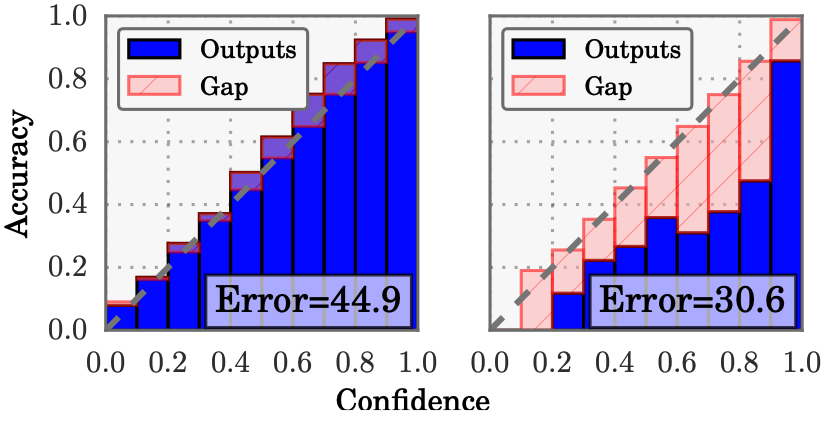
\includegraphics[width=\textwidth]{figures/nn-calibration}
        \end{column}
        \begin{column}{0.5\textwidth}
            \begin{itemize}
                \item Modern neural networks are poorly calibrated \href{https://arxiv.org/pdf/1706.04599.pdf}{[Gao et al., 2017]}
                \item Left: 5 layer LeNet
                \item Right: 110 layer ResNet
            \end{itemize}
        \end{column}
    \end{columns}
\end{frame}

\begin{frame}
    {ECE calculation example}

    Practicalities:\\
    \begin{itemize}
        \item Number of bins can have large impact on the calculated ECE\pause
        \item Some bins may contain very few examples 
        \item Equally sized bins are also used in practice
    \end{itemize}

    \vspace{-1em}
    \begin{figure}
        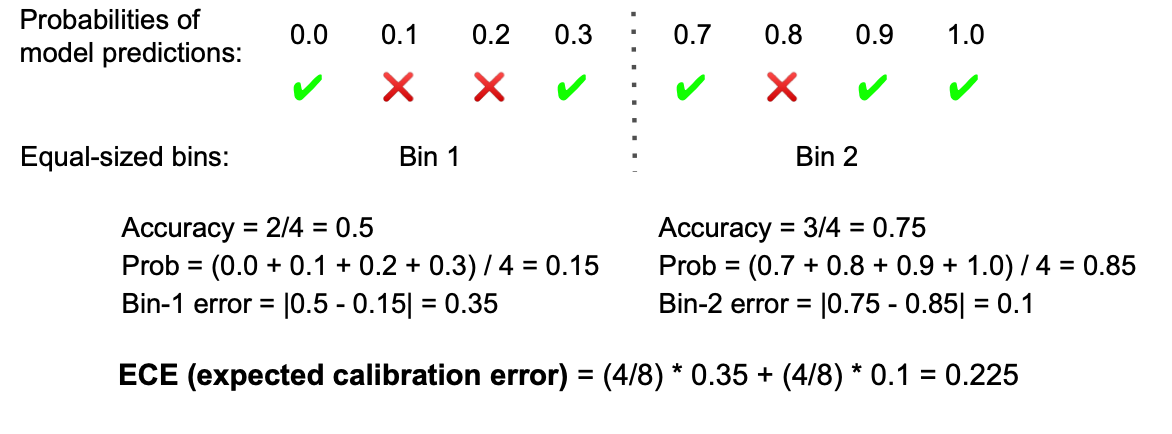
\includegraphics[height=4cm]{figures/ece-calc}
        \caption{From \href{https://arxiv.org/pdf/2211.09110.pdf}{HELM}}
    \end{figure}
\end{frame}

\begin{frame}
    {Selective classification}
    How can we use the confidence score?\\
    \begin{itemize}
    \item Abstain (not predicting) on examples with low confidence
        \item Optionally ask for human help
    \end{itemize}

    \pause
    Concept check: given a perfectly calibrated model, if we abstain on examples whose confidence score is below 0.8, what's the accuracy we will get?

    \pause
    \textbf{Accuracy-coverage trade-off}:\\
    \begin{itemize}
    \item Accuracy can be improved by raising the confidence threshold
    \item But coverage (fraction of examples where we make a prediction) is reduced with increasing threshold
    \end{itemize}
\end{frame}

\begin{frame}
    {Selective classification metrics}

    \textbf{Accuracy at a specific coverage}
    \begin{figure}
        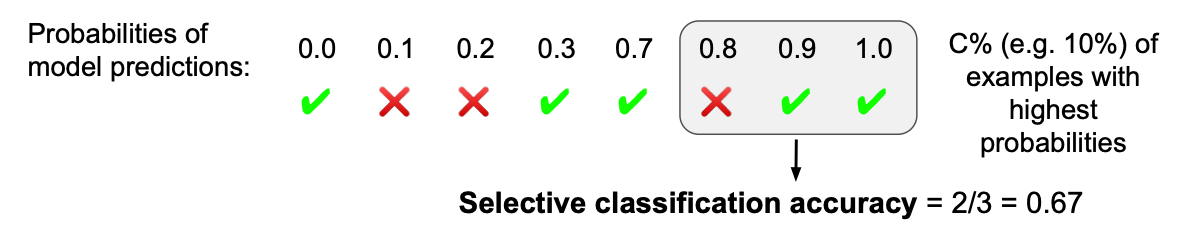
\includegraphics[width=\textwidth]{figures/sel-class}
        \caption{From \href{https://arxiv.org/pdf/2211.09110.pdf}{HELM}}
    \end{figure}
    \pause

    \textbf{Area under the accuracy-coverage curve}: average accuracy at different coverage

\end{frame}

\begin{frame}
    {Does LM know what it doesn't know?}
    \begin{figure}
        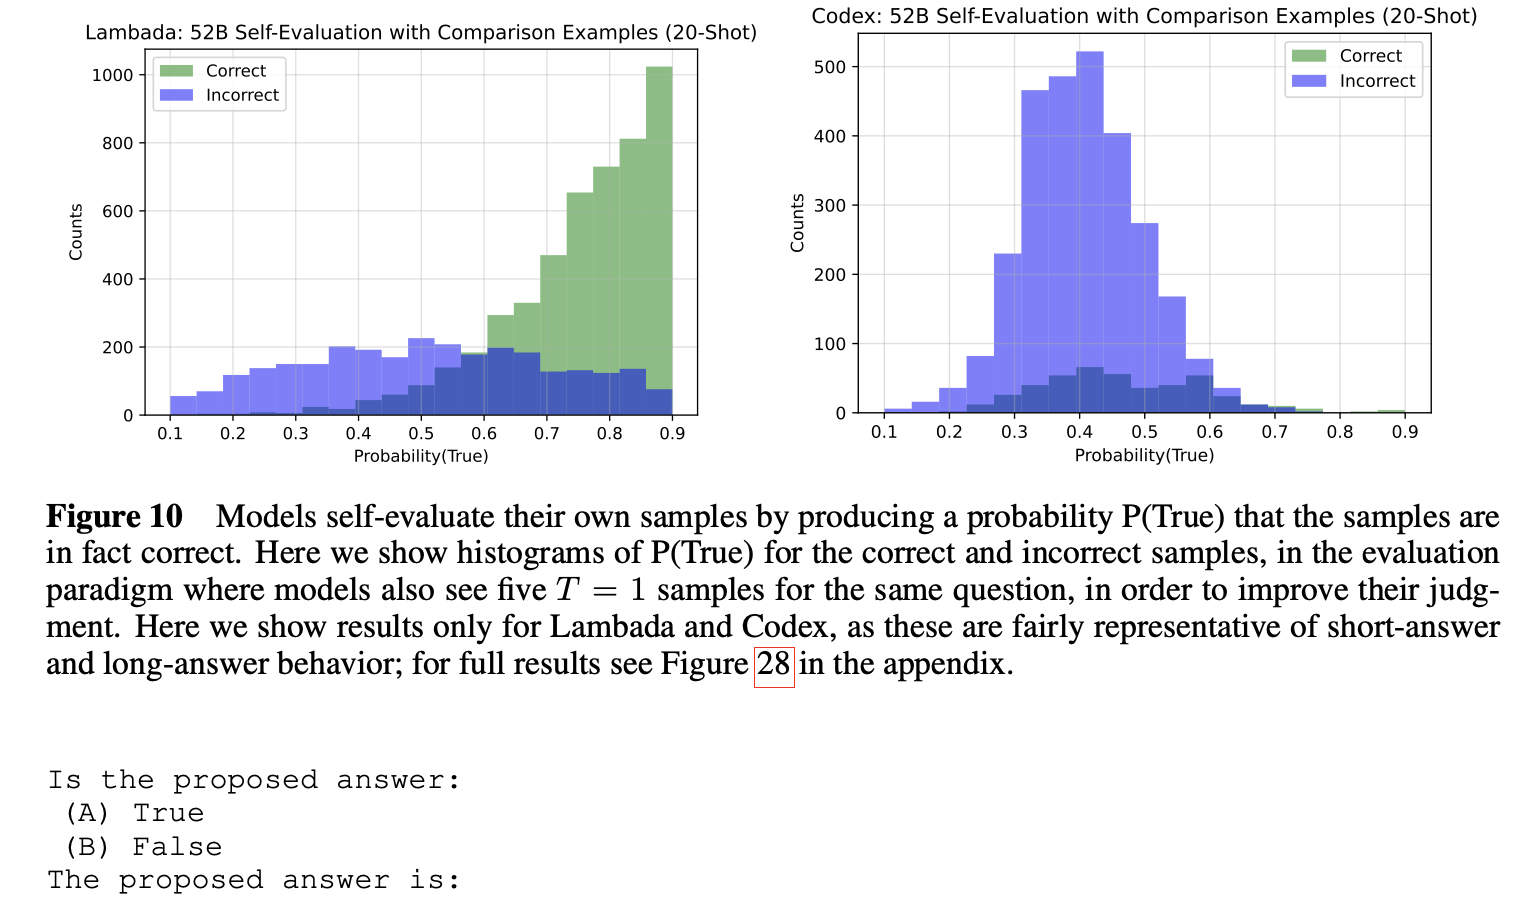
\includegraphics[width=.9\textwidth]{figures/lm-know}
        \caption{From \mycite[https://arxiv.org/pdf/2207.05221]{Kadavath et al., 2022}}
    \end{figure}
\end{frame}


\begin{frame}
    {Privacy}

    Models are now trained on large quantities of \textit{public} internet data.

    What could be the privacy concerns?\\\pause
    \begin{itemize}[<+->]
        \item Private data can be leaked to the internet
        \item Private data can be inferred by linking multiple public data sources
        \item Private data can be predicted from public information
        \item Sensitive public information can be shared more widely out of the intended context
    \end{itemize}
\end{frame}

\begin{frame}
    {Can we extracting sensitive data from models?}
    Models can generate its training data verbatim \href{https://arxiv.org/pdf/2012.07805.pdf}{[Carlini et al., 2021]}:\vspace{-1.5em}
    %\begin{columns}
    %    \begin{column}{0.5\textwidth}
    %        \begin{figure}
    %        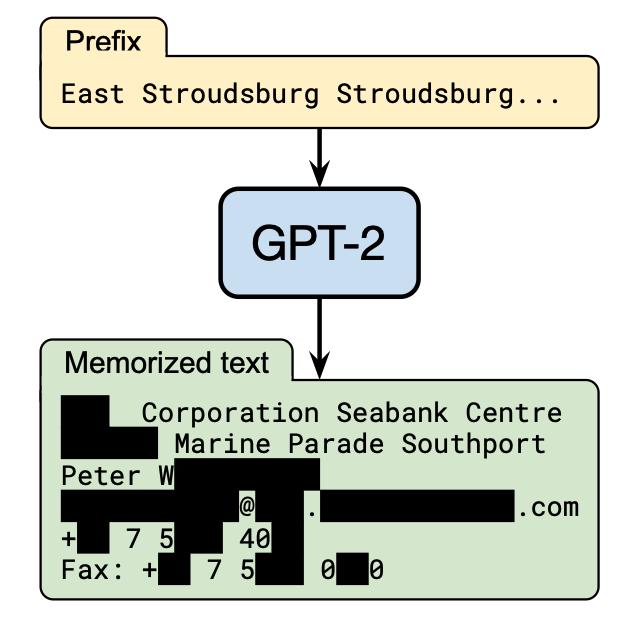
\includegraphics[width=0.9\textwidth]{figures/mem-gpt2}
    %        \end{figure}
    %    \end{column}
    %    \begin{column}{0.5\textwidth}
    %        \begin{figure}
    %        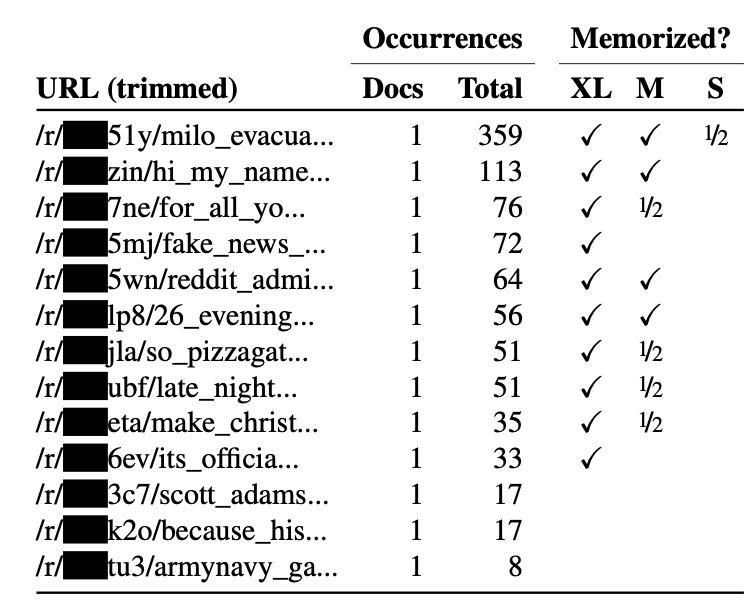
\includegraphics[width=\textwidth]{figures/mem-gpt2-string}
    %        \end{figure}
    %    \end{column}
    %    \end{columns}
            \begin{figure}
            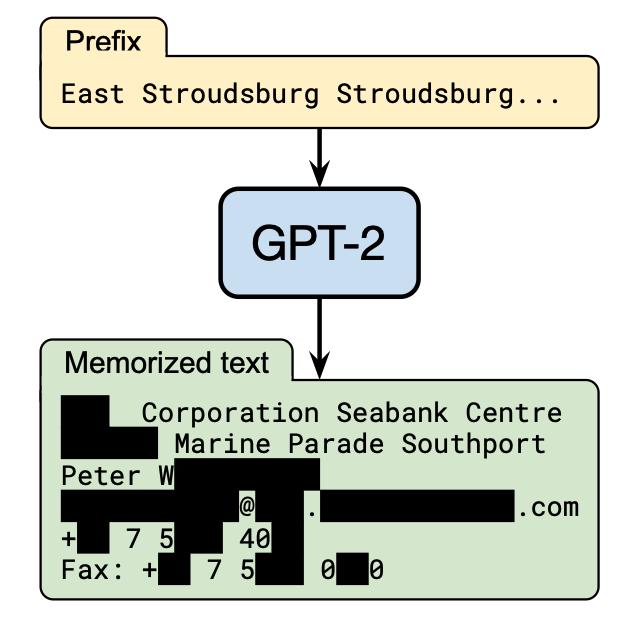
\includegraphics[height=0.5\textheight]{figures/mem-gpt2}
            
\includegraphics[width=0.9\textwidth]{figures/peter}
            \end{figure}
\end{frame}

\begin{frame}
    {How to extract memorized data from models?}
            \begin{figure}
            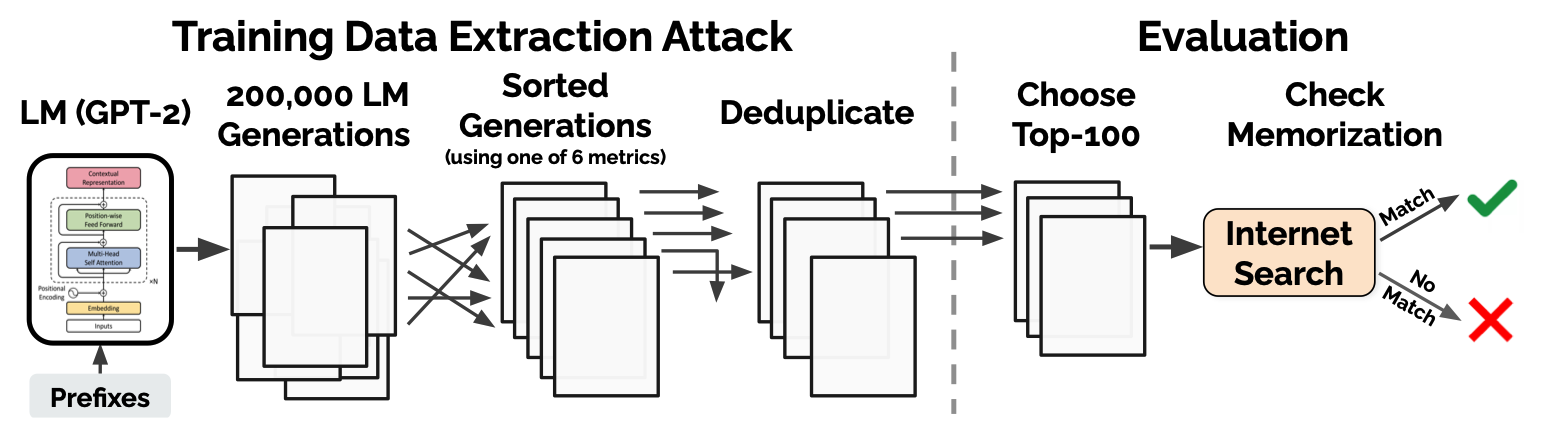
\includegraphics[width=0.8\textwidth]{figures/mem-gpt2-method}
            \end{figure}
            \vspace{-2em}

            How to find potentially memorized text?\\
            \begin{itemize}
                \item Direct sampling would produce common text (e.g., I don't know)
            \pause
                \item \textbf{Key idea}: compare to a second model; text is `interesting' if its likelihood is only high under the original model.
                    \begin{itemize}
                        \item likelihood under a smaller model 
                        \item zlib compression entropy (effective at removing repeated strings)
                        \item likelihood of lowercased text 
                    \end{itemize}
            \end{itemize}
\end{frame}

\begin{frame}
    {What kind of data can be extracted?}
    \begin{columns}
        \begin{column}{0.5\textwidth}
            \begin{figure}
            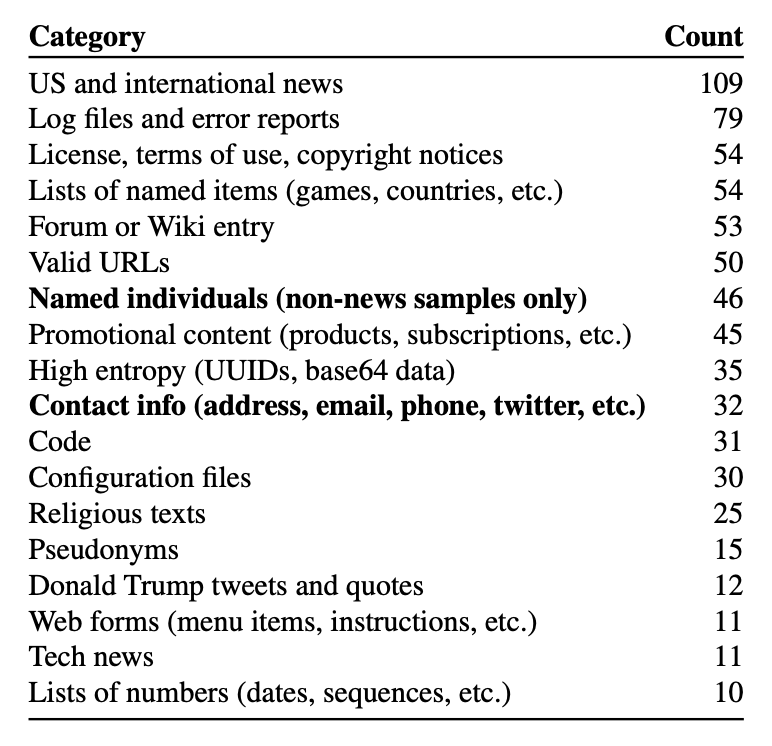
\includegraphics[width=\textwidth]{figures/mem-data}
            \end{figure}
        \end{column}
        \begin{column}{0.5\textwidth}
            Repeated data is more likely to be extracted:
            \begin{figure}
            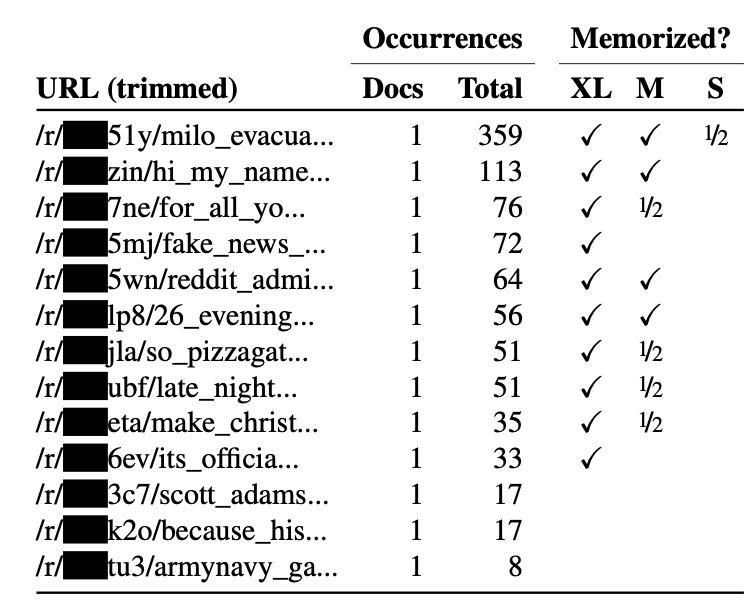
\includegraphics[width=\textwidth]{figures/mem-gpt2-string}
            \end{figure}
        \end{column}
        \end{columns}
\end{frame}

% TODO: data contamination

%\begin{frame}
%    {Summary}
%    \begin{itemize}
%        \item Privacy: the user has the right to be left out
%        \item Highly relevant when training on internet-scale data
%            \begin{itemize}
%                \item Memorizing copyrighted text, e.g., books, code
%                \item Memorizing personally identifiable information
%            \end{itemize}
%        \item Lots of open questions:
%            \begin{itemize}
%                \item What kind of data is considered private / sensitive?
%                \item Definition of privacy (DP, verbatim memorization...)
%                \item How to unlearn a user's data after training on it? 
%            \end{itemize}
%    \end{itemize}
%\end{frame}

\end{document}
